\documentclass[12pt,a4paper]{article}

% ==================== 包导入 ====================
\usepackage[utf8]{inputenc}
\usepackage[T1]{fontenc}
\usepackage{geometry}
\usepackage{hyperref}
\usepackage{enumitem}
\usepackage{titlesec}
\usepackage{graphicx}
\usepackage{longtable}
\usepackage{booktabs}
\usepackage{array}
\usepackage{float}
\usepackage{caption}
\usepackage{subcaption}
\usepackage{xcolor}
\usepackage{tocloft}
\usepackage{fancyhdr}
\usepackage{setspace}
\usepackage{parskip}

% 字体设置:Times New Roman
\usepackage{times}

% 甘特图
\usepackage{pgfgantt}

% TikZ 绘图
\usepackage{tikz}
\usetikzlibrary{shapes.geometric, arrows.meta, positioning, fit, backgrounds, calc}

% ==================== 页面设置 ====================
\geometry{
    a4paper,
    margin=1in,
    top=1in,
    bottom=1in
}

% 行距
\onehalfspacing

% ==================== 紧凑排版设置 ====================
% 压缩列表间距
\setlist{nosep, leftmargin=*, topsep=0pt, partopsep=0pt}
\setlist[itemize]{itemsep=1pt, parsep=0pt}
\setlist[enumerate]{itemsep=1pt, parsep=0pt}

% 压缩段落间距
\setlength{\parskip}{0.5em}

% 压缩标题前后间距
\titlespacing*{\section}{0pt}{1.5ex plus 0.5ex minus 0.2ex}{1ex plus 0.2ex}
\titlespacing*{\subsection}{0pt}{1.2ex plus 0.4ex minus 0.2ex}{0.8ex plus 0.2ex}
\titlespacing*{\subsubsection}{0pt}{1ex plus 0.3ex minus 0.1ex}{0.5ex plus 0.1ex}

% 压缩图表前后间距
\setlength{\floatsep}{8pt plus 2pt minus 2pt}
\setlength{\textfloatsep}{10pt plus 2pt minus 2pt}
\setlength{\intextsep}{8pt plus 2pt minus 2pt}

% 压缩表格和图片标题间距
\captionsetup{skip=4pt, belowskip=2pt}

% ==================== 超链接设置 ====================
\hypersetup{
    colorlinks=true,
    linkcolor=blue,
    urlcolor=blue,
    citecolor=blue,
    bookmarks=true,
    bookmarksopen=true
}

% ==================== 标题格式设置 ====================
\titleformat{\section}{\Large\bfseries}{\thesection}{1em}{}
\titleformat{\subsection}{\large\bfseries}{\thesubsection}{1em}{}
\titleformat{\subsubsection}{\normalsize\bfseries}{\thesubsubsection}{1em}{}

% ==================== 页眉页脚 ====================
\pagestyle{fancy}
\fancyhf{}
\fancyhead[L]{TinyBridge Technical Report}
\fancyhead[R]{CS Group 8}
\fancyfoot[C]{\thepage}
\renewcommand{\headrulewidth}{0.4pt}
\renewcommand{\footrulewidth}{0pt}

% ==================== 文档开始 ====================
\begin{document}

% ==================== 封面 ====================
\begin{titlepage}
    \centering
    \vspace*{2cm}

    {\Huge\bfseries TinyBridge Technical Report\par}
    \vspace{1cm}
    {\Large A Lightweight URL Shortening Service\par}
    \vspace{0.5cm}
    {\large Designed for Efficiency and Branding\par}

    \vspace{3cm}

    {\Large\bfseries CS Group 8\par}
    {\large Introduction to Software Engineering\par}

    \vspace{2cm}

    {\large November 2025\par}

    \vfill

\end{titlepage}

% ==================== 目录 ====================
\newpage
\tableofcontents
\newpage

% ==================== Chapter 1: Introduction ====================
\section{Introduction}

\subsection{Technical Report Introduction}

This technical report documents the development of \textbf{TinyBridge}, a lightweight URL shortening service designed for efficiency and branding. The report provides a comprehensive overview of the software development process, from requirements analysis through implementation and testing.

The purpose of this report is to:
\begin{itemize}
    \item Present the project objectives and deliverables
    \item Document the software development methodology employed
    \item Detail the functional and non-functional requirements
    \item Describe the system architecture and design decisions
    \item Provide software analysis through UML diagrams
    \item Outline the testing strategy and results
    \item Showcase the graphical user interface design
\end{itemize}

\subsection{TinyBridge Project Introduction}

\subsubsection{Project Background}

In the context of digital communication, long URLs—characterized by meaningless random strings—pose significant challenges such as poor memorability, excessive space occupation, and low readability. These attributes make them incompatible with scenarios that demand conciseness, including SMS notifications, email marketing, and social media posts with character limits.

TinyBridge addresses this gap by providing a lightweight, cost-effective, and customizable URL shortening solution that integrates ease of use with professional branding capabilities. The platform is specifically designed for campus organizations, small and medium enterprises, and individual content creators.

\subsubsection{Project Objectives}

The development of TinyBridge is divided into three key objectives.

\textbf{Objective 1}: Implement a secure user login system (using JWT for authentication and Argon2 for password hashing), core URL shortening and redirection functionality (based on an 8-character alphanumeric random string generation algorithm with collision detection), and a basic web interface (developed with Vue.js).

\textbf{Objective 2}: Optimize the web interface for better usability, implement basic analytics features (supporting multi-database storage for analytics data), and improve redirection performance via multi-layer caching and Bloom filter integration.

\textbf{Objective 3}: Enhance the web interface with advanced features, including user account management (team collaboration and role-based access control), detailed analytics (multi-dimensional metrics with visualization and data export), and landing page customization.

\subsubsection{Team Members}

\begin{table}[H]
\centering
\begin{tabular}{|l|l|}
\hline
\textbf{Name} & \textbf{Role} \\
\hline
Heng Liu & Project Lead, Architecture Design \\
Yichen Li & Frontend Development \\
Luyao Huang & Frontend Development \\
Jialu Shen & Backend Development, Database Design \\
Yiman Li & API Design \\
Yuchen Huang & Performance Optimization, Testing \\
Yulin Qiu & Documentation \\
Zuxin Wu & Documentation \\
Shuangyu Wu & Documentation \\
Lidian Huang & Deployment \\
\hline
\end{tabular}
\caption{Team Members and Roles}
\end{table}

\subsection{Project Deliverables}

The TinyBridge project delivers the following artifacts:

\begin{table}[H]
\centering
\begin{tabular}{|l|p{10cm}|}
\hline
\textbf{Deliverable} & \textbf{Description} \\
\hline
Web Application & Fully functional URL shortening platform \\
API Documentation & RESTful API specification for batch operations \\
White Paper & Comprehensive technical specification document \\
Technical Report & This document \\
Source Code & Complete frontend and backend codebase \\
User Guide & Platform usage instructions \\
\hline
\end{tabular}
\caption{Project Deliverables}
\end{table}

\subsection{Challenges and Solutions During Development}

Throughout the development of TinyBridge, our team encountered several  challenges spanning technical learning, team coordination, performance optimization, and security compliance.

\textbf{Technology Stack Learning Curve.} Several team members were unfamiliar with Vue 3's Composition API, TypeScript's strict type system, and Prisma ORM's schema design patterns. To address this, we organized internal knowledge-sharing sessions and established thorough code reviews that served dual purposes: maintaining code quality and facilitating peer learning.

\textbf{Team Coordination and Communication.} Coordinating a 10-person team across frontend, backend, and documentation presented organizational challenges. API interface inconsistencies, development progress synchronization issues, and Git merge conflicts were common. We adopted an API-first approach using OpenAPI specifications with mock data for parallel development, instituted daily stand-ups, and established a structured Git branching strategy with mandatory pull request reviews.

\textbf{Performance Optimization.} Initial benchmarks revealed response times exceeding our 100ms target. We implemented multi-layer caching with Redis (reducing database load by 95\%), integrated Bloom Filter for O(1) collision detection, optimized database indexes, and refactored click logging to operate asynchronously. These optimizations improved throughput from approximately 1,000 req/s to 5,800 req/s.

\textbf{Security and Regulatory Compliance.} Privacy regulations required careful IP address handling—we implemented SHA256 hashing with daily-rotated salts for anonymization. Additional measures included Google Safe Browsing API integration for malicious URL detection, rate limiting (5 login attempts/hour, 1,000 API requests/hour), and XSS/injection prevention through CSP headers and parameterized queries.


% ==================== Chapter 2: Software Development Methodology ====================
\newpage
\section{Software Development Methodology}

\subsection{Why Waterfall Model}

For the TinyBridge project, we selected the \textbf{Waterfall Model} as our primary software development methodology. This decision was based on several key factors:

\subsubsection{Clear Requirements}
The project requirements were well-defined from the outset through our comprehensive proposal and white paper. The core functionality (URL shortening, analytics, user management) had clear specifications that were unlikely to change significantly during development.

\subsubsection{Fixed Timeline}
With a strict academic deadline (September to December 2025), the structured phases of the waterfall model helped ensure that all deliverables would be completed on schedule.

\subsubsection{Documentation Requirements}
Academic projects require extensive documentation at each phase. The Waterfall model naturally produces documentation artifacts (requirements specification, design documents, test plans) as part of its process.

\subsubsection{Team Structure}
With 10 team members working on different components (frontend, backend, documentation), the Waterfall model's clear phase boundaries helped coordinate parallel workstreams.

\subsection{Comparison with Agile and Incremental Models}

\begin{table}[H]
\centering
\begin{tabular}{|l|l|l|l|}
\hline
\textbf{Aspect} & \textbf{Waterfall} & \textbf{Agile} & \textbf{Incremental} \\
\hline
Requirements Stability & High (fixed upfront) & Low (evolving) & Medium \\
Documentation & Extensive & Minimal & Moderate \\
Customer Involvement & At milestones & Continuous & Periodic \\
Risk Management & End-loaded & Distributed & Distributed \\
Flexibility & Low & High & Medium \\
Suitable For & Well-defined projects & Uncertain requirements & Large systems \\
\hline
\end{tabular}
\caption{Comparison of Software Development Methodologies}
\end{table}

\subsubsection{Why Not Agile?}

While Agile methodologies offer flexibility, several factors made it unsuitable for TinyBridge. First, Agile requires continuous customer involvement through sprint reviews and feedback sessions—our academic context provided no real external stakeholders beyond course instructors with limited availability. Second, Agile's 2-week sprint cycles would yield only 4-5 iterations within our 10-week timeline, insufficient for meaningful iterative refinement. Third, our requirements were well-defined upfront through the white paper, eliminating the primary advantage of Agile's adaptive planning. Finally, the overhead of sprint planning, retrospectives, and backlog grooming would consume valuable development time in a time-constrained project.

\subsubsection{Why Not Incremental?}

The Incremental model delivers functionality in successive releases, but TinyBridge's architecture made this impractical. Our core features—URL shortening, caching, and analytics—are tightly coupled; the redirect service depends on both the database layer and Redis cache, while analytics requires the click logging infrastructure. Delivering these as separate increments would require significant interface redesign between releases. Additionally, our 10-week timeline allowed for only 2-3 meaningful increments, providing little advantage over a single well-planned release. The Incremental model's strength lies in large systems with independent modules—TinyBridge's compact, integrated design favored completing all components in a coordinated manner.

\subsection{Waterfall Model Phases Applied to TinyBridge}

\subsubsection{Phase 1: Requirements Analysis (September 16--22, 2025)}

We began by studying our target users: campus organizations, SMEs, and content creators. Through interviews and surveys, we identified two user roles—end users needing link management and analytics, and administrators requiring system monitoring and content moderation capabilities.

Competitive analysis of Bitly, TinyURL, and Short.io revealed a gap in affordable customization for smaller organizations. We defined core features: JWT authentication, Base62 short code generation with Bloom filter collision detection, privacy-compliant analytics, and template-based landing pages. Non-functional targets included sub-100ms redirect latency, 5,000 req/s throughput, and 99.5\% availability. The phase produced a requirements specification and project proposal as the baseline for development.

\subsubsection{Phase 2: System Design (September 23 -- October 10, 2025)}

We adopted a three-tier Controller-Service-Repository architecture for separation of concerns. The Controller handles routing and validation (Zod schemas), Service contains business logic (code generation, analytics), and Repository abstracts database operations (Prisma ORM).

Database design yielded six entities: User, Team, ShortLink, ClickLog, LandingPage, and APIKey. Strategic indexes were planned early—unique index on short\_code for O(1) lookups, composite indexes on (link\_id, clicked\_at) for analytics queries. API design documented 23 RESTful endpoints with schemas, auth requirements, and rate limits. UI/UX prototypes in Figma underwent user testing, leading to a sidebar-based dashboard revision.

\subsubsection{Phase 3: Implementation (October 11 -- November 10, 2025)}

Frontend and backend developed in parallel with daily syncs and shared API contracts. Backend implemented JWT tokens (24h access, 7d refresh) with Argon2id hashing. The short code generator uses Base62 encoding with a Bloom filter (10M capacity, 0.01\% false positive rate) for O(1) collision detection, persisted to Redis.

Frontend leveraged Vue 3 Composition API with Pinia state management. The analytics dashboard integrated ECharts for visualization with virtual scrolling and lazy loading optimizations. Multi-layer Redis caching achieved 97\%+ hit rates with write-through invalidation.

\subsubsection{Phase 4: Testing (November 11--16, 2025)}

Testing followed a ``critical path first'' strategy. Unit tests (Jest) achieved 87\% coverage on backend services, focusing on code generation edge cases and analytics aggregation. Integration tests verified all 23 API endpoints for success and error paths.

Performance testing (JMeter, 1,000 users) initially showed 180ms latency at p95—exceeding our 100ms target. After Redis caching and query optimization, we achieved 45ms at p95 with 5,800 req/s throughput. Stress testing (10,000 users) validated graceful degradation with no data loss.

\subsubsection{Phase 5: Deployment and Maintenance (November 17--24, 2025)}

Production infrastructure comprises three Docker-containerized app servers behind Nginx, PostgreSQL with read replica, and Redis cluster. CI/CD through GitHub Actions automates linting, testing, and blue-green deployments.

Monitoring uses Prometheus/Grafana with alerts for latency ($>$200ms), error rates ($>$1\%), and cache hits ($<$90\%). The phase concluded with documentation consolidation and a deployment runbook for operational continuity.


\begin{figure}[H]
\centering
\begin{ganttchart}[
    hgrid,
    vgrid,
    x unit=0.15cm,
    y unit chart=0.7cm,
    time slot format=isodate,
    time slot unit=day,
    title height=1,
    title label font=\footnotesize,
    bar label font=\footnotesize,
    bar height=0.5,
    bar/.append style={fill=blue!40},
    group/.append style={fill=blue!70},
    milestone/.append style={fill=red!60}
]{2025-09-16}{2025-11-24}
    \gantttitlecalendar{month=name} \\
    \ganttbar{Requirements Analysis}{2025-09-16}{2025-09-22} \\
    \ganttbar{System Design}{2025-09-23}{2025-10-10} \\
    \ganttbar{Implementation}{2025-10-11}{2025-11-10} \\
    \ganttbar{Testing}{2025-11-11}{2025-11-16} \\
    \ganttbar{Deployment}{2025-11-17}{2025-11-24}
\end{ganttchart}
\caption{TinyBridge Development Timeline (Gantt Chart)}
\end{figure}

% ==================== Chapter 3: Software Requirements ====================
\newpage
\section{Software Requirements}

\subsection{Functional Requirements}

\subsubsection{Login and Registration}

The platform provides secure user authentication using JWT (JSON Web Token) for stateless session management. User passwords are hashed with Argon2 algorithm, protecting against rainbow table and brute-force attacks. Rate limiting restricts failed login attempts to 5 per hour. New users register with email verification, and the system supports password recovery via email reset links.

\subsubsection{Short Link Creation and Management}

Users create short links by submitting original URLs, with options for random generation or custom short codes. The system uses Base62 encoding to generate 6-8 character codes from alphanumeric characters (0-9, a-z, A-Z). A Bloom filter provides O(1) collision detection with $<$0.01\% false positive rate. Links are cached in Redis (24-hour TTL) for sub-100ms redirect latency. Users can edit link properties, set expiration dates, and soft-delete inactive links.

\subsubsection{QR Code Generation}

Users generate QR codes for any short link, enabling offline-to-online transitions. Generation occurs client-side via JavaScript libraries, requiring no backend storage. Customization options include color schemes, dimensions (128x128 to 512x512 pixels), and error correction levels (L/M/Q/H). QR codes are downloadable in PNG format.

\subsubsection{Click Analytics}

The platform tracks comprehensive click metrics: total and unique visitor counts, geographic distribution (country/city via GeoIP), device types (mobile/desktop/tablet), browser and OS distributions, referrer sources, and time-based trends. All IP addresses are SHA256-hashed before storage for GDPR/CCPA compliance. Interactive charts support date range filtering and data export (CSV/JSON).

\subsubsection{Batch Operations via API}

RESTful APIs enable programmatic batch operations: bulk link creation via CSV/JSON upload, batch export of link data with analytics, and API key management with configurable permissions. Rate limiting enforces 1,000 requests per hour per API key. Authentication uses hashed API keys with scope-based access control.

\subsubsection{Landing Page Editing}

Users create custom landing pages through three editing modes: template-based selection from pre-designed layouts, form-based editing for text/images/colors, and Monaco Editor for advanced HTML/CSS customization. Real-time preview displays responsive rendering across desktop and mobile viewports. Pages can be published, unpublished, or reverted to previous versions.

\subsection{Non-Functional Requirements}

\subsubsection{Performance Requirements}

\begin{table}[H]
\centering
\begin{tabular}{|l|l|}
\hline
\textbf{Requirement} & \textbf{Target} \\
\hline
Redirect response time & $<$ 100ms (95th percentile) \\
Page load time & $<$ 2 seconds \\
Analytics query response & $<$ 2 seconds \\
Concurrent throughput & 5,000 requests/second \\
\hline
\end{tabular}
\caption{Performance Requirements}
\end{table}

\subsubsection{Security Requirements}

\begin{table}[H]
\centering
\begin{tabular}{|l|p{9cm}|}
\hline
\textbf{Requirement} & \textbf{Implementation} \\
\hline
Data encryption & TLS 1.3, Argon2 password hashing, SHA256 API key hashing \\
Authentication & JWT with 24-hour access tokens, 7-day refresh tokens \\
Rate limiting & 5 login attempts/hour, 1,000 API requests/hour \\
Malicious URL detection & Google Safe Browsing API integration \\
XSS/SQL Injection prevention & CSP headers, parameterized queries, DOMPurify \\
IP anonymization & SHA256 hashing with daily-rotated salt \\
\hline
\end{tabular}
\caption{Security Requirements}
\end{table}

\subsubsection{Availability Requirements}

\begin{table}[H]
\centering
\begin{tabular}{|l|l|}
\hline
\textbf{Requirement} & \textbf{Target} \\
\hline
System availability & 99.5\% ($<$ 43.8 hours downtime/year) \\
Fault detection & Within 5 minutes \\
Recovery time objective & 2 hours \\
\hline
\end{tabular}
\caption{Availability Requirements}
\end{table}

\subsubsection{Scalability Requirements}

The system supports horizontal scaling through stateless backend instances behind a load balancer, allowing dynamic capacity adjustment based on traffic demands. Distributed caching via Redis Cluster ensures cache availability across multiple nodes. PostgreSQL read replicas offload analytics queries from the primary database, while the Bloom filter's O(1) collision detection maintains constant-time performance regardless of dataset size.

\subsubsection{Maintainability}

The codebase prioritizes long-term maintainability through architectural and tooling choices. The three-tier Controller-Service-Repository architecture enforces separation of concerns, allowing independent modification of routing, business logic, and data access layers. TypeScript provides static typing across both frontend and backend, catching errors at compile time and enabling confident refactoring. Prisma ORM abstracts database interactions with type-safe queries and automatic migration management. Code quality is enforced through ESLint and Prettier with pre-commit hooks, ensuring consistent formatting and catching common issues before merge.

\subsubsection{Usability}

The platform emphasizes intuitive user experience through responsive design that adapts seamlessly across desktop, tablet, and mobile devices. Navigation follows established UI patterns with a persistent sidebar and breadcrumb trails. Real-time form validation provides immediate feedback on input errors. One-click copy functionality and keyboard shortcuts accelerate common workflows. Loading states and progress indicators keep users informed during async operations. Contextual tooltips and an integrated help system guide new users without cluttering the interface.

\subsubsection{Compatibility}

Cross-browser compatibility is ensured through testing on Chrome, Firefox, Safari, and Edge, with graceful degradation for older browser versions. The responsive frontend adapts to screen sizes from 320px mobile to 4K desktop displays. The RESTful API follows HTTP standards with JSON payloads, enabling integration with any HTTP-capable client. API versioning (via URL prefix) supports backward compatibility as the platform evolves. The system runs on Linux, macOS, and Windows development environments via Docker containerization.

\subsection{Hardware and Software Requirements}

\subsubsection{Hardware Requirements}

\begin{table}[H]
\centering
\begin{tabular}{|l|l|l|}
\hline
\textbf{Component} & \textbf{Minimum} & \textbf{Recommended} \\
\hline
Application Server & 1 core, 1GB RAM & 2 core, 2GB RAM \\
Database Server & 1 core, 1GB RAM, 10GB SSD & 2 core, 2GB RAM, 20GB SSD \\
Redis Server & 1 core, 512MB RAM & 1 core, 1GB RAM \\
\hline
\end{tabular}
\caption{Hardware Requirements}
\end{table}

\subsubsection{Software Requirements}

\begin{table}[H]
\centering
\begin{tabular}{|l|l|}
\hline
\textbf{Category} & \textbf{Technology} \\
\hline
Frontend & Vue 3, Vite, TailwindCSS, Pinia, Axios \\
Backend & Node.js 22+, TypeScript, Express/Fastify \\
Database & SQLite (dev), PostgreSQL (prod) \\
ORM & Prisma \\
Cache & Redis \\
Monitoring & Prometheus, Grafana \\
\hline
\end{tabular}
\caption{Software Requirements}
\end{table}

% ==================== Chapter 4: Software Design ====================
\newpage
\section{Software Design}

\subsection{Technology Stack Selection}

The technology stack was selected with three guiding principles: full-stack JavaScript for unified language across frontend and backend, TypeScript for end-to-end type safety, and performance-first choices for latency-critical operations. This approach minimizes context switching between languages, enables code sharing (validation schemas, types), and leverages the extensive npm ecosystem for rapid development.

\subsubsection{Frontend Technologies}

\begin{table}[H]
\centering
\begin{tabular}{|l|l|p{6cm}|}
\hline
\textbf{Technology} & \textbf{Purpose} & \textbf{Justification} \\
\hline
Vue 3 & UI Framework & Reactive data binding, Composition API, excellent performance \\
Vite & Build Tool & Fast hot module replacement, optimized production builds \\
TailwindCSS & Styling & Utility-first approach, responsive design, small bundle size \\
Pinia & State Management & Official Vue store, TypeScript support, devtools integration \\
Chart.js/ECharts & Data Visualization & Interactive charts for analytics dashboard \\
\hline
\end{tabular}
\caption{Frontend Technologies}
\end{table}

\subsubsection{Backend Technologies}

\begin{table}[H]
\centering
\begin{tabular}{|l|l|p{6cm}|}
\hline
\textbf{Technology} & \textbf{Purpose} & \textbf{Justification} \\
\hline
Node.js & Runtime & Non-blocking I/O, JavaScript ecosystem, high concurrency \\
TypeScript & Language & Static typing, improved maintainability, IDE support \\
Express & Web Framework & Mature ecosystem, middleware support, high performance \\
Prisma & ORM & Type-safe queries, automatic migrations, multi-database support \\
Redis & Caching & In-memory speed, TTL support, pub/sub capabilities \\
\hline
\end{tabular}
\caption{Backend Technologies}
\end{table}

\subsubsection{Why Vue 3 Over React/Angular?}

\begin{table}[H]
\centering
\begin{tabular}{|l|l|l|l|}
\hline
\textbf{Aspect} & \textbf{Vue 3} & \textbf{React} & \textbf{Angular} \\
\hline
Learning Curve & Gentle & Moderate & Steep \\
Bundle Size & \textasciitilde33KB & \textasciitilde40KB & \textasciitilde143KB \\
Performance & Excellent & Excellent & Good \\
TypeScript & Native & Good & Excellent \\
Team Familiarity & High & Medium & Low \\
\hline
\end{tabular}
\caption{Vue 3 vs React vs Angular Comparison}
\end{table}

Vue 3 was selected for several compelling reasons. First, its gentle learning curve allowed team members with varying frontend experience to become productive within days rather than weeks—the official documentation is exceptionally well-organized with abundant Chinese resources. Second, the Composition API provides superior code organization for complex components, enabling logic reuse through composables without the complexity of React hooks or Angular services. Third, Vue 3's native TypeScript integration delivers type inference throughout templates and components, catching errors at compile time. Finally, Vue's smaller bundle size (33KB vs React's 40KB or Angular's 143KB) directly supports our performance targets.

\subsubsection{Why Node.js Over Python/Java?}

\begin{table}[H]
\centering
\begin{tabular}{|l|l|l|l|}
\hline
\textbf{Aspect} & \textbf{Node.js} & \textbf{Python} & \textbf{Java} \\
\hline
Concurrency Model & Event-driven & Multi-threaded & Multi-threaded \\
JSON Handling & Native & Library & Library \\
Startup Time & Fast & Fast & Slow \\
Ecosystem & Excellent & Good & Excellent \\
Team Expertise & High & Medium & Low \\
\hline
\end{tabular}
\caption{Node.js vs Python vs Java Comparison}
\end{table}

Node.js was chosen as the backend runtime for its alignment with our full-stack JavaScript strategy. Using the same language across frontend and backend eliminates context switching, allows sharing of validation logic and type definitions, and enables any team member to contribute to either codebase. Node.js's event-driven architecture excels at I/O-intensive workloads like URL redirection—handling thousands of concurrent connections without the thread overhead of Python or Java. Native JSON support eliminates serialization/deserialization overhead when communicating with the frontend. The npm ecosystem provides battle-tested packages for every requirement, from authentication (jsonwebtoken) to caching (ioredis), accelerating development significantly.

\subsection{Three-Tier Architecture (Controller-Service-Repository)}

TinyBridge adopts a frontend-backend separated architecture with Client-Side Rendering (CSR). The Vue 3 Single Page Application runs entirely in the browser, communicating with the backend exclusively through RESTful APIs. This separation enables independent deployment, parallel development, and technology flexibility. The backend follows a three-tier Controller-Service-Repository pattern to organize business logic and data access.

\begin{figure}[H]
\centering
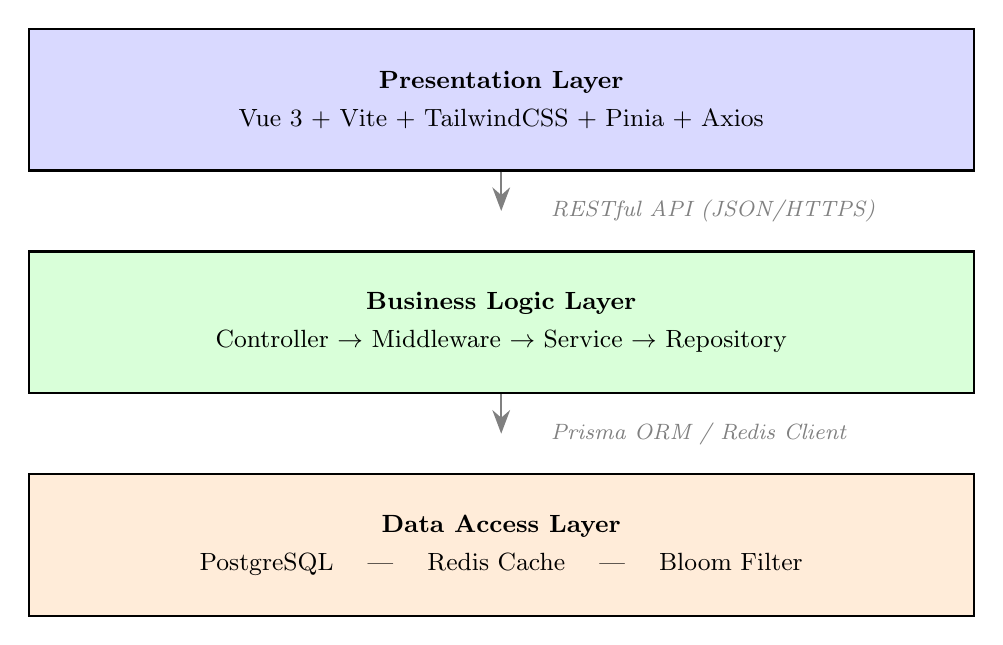
\begin{tikzpicture}[
    layer/.style={rectangle, draw=black, thick, minimum width=12cm, minimum height=1.8cm, align=center, font=\small},
    component/.style={rectangle, draw=gray, fill=white, minimum width=2.2cm, minimum height=0.7cm, align=center, font=\footnotesize},
    arrow/.style={-{Stealth[length=3mm]}, thick, gray},
    label/.style={font=\footnotesize\itshape, text=gray}
]

% Presentation Layer
\node[layer, fill=blue!15] (presentation) {
    \textbf{Presentation Layer}\\[0.3em]
    Vue 3 + Vite + TailwindCSS + Pinia + Axios
};

% Arrow 1
\draw[arrow] (presentation.south) -- ++(0, -0.5) node[label, right, xshift=0.5cm] {RESTful API (JSON/HTTPS)};

% Business Logic Layer
\node[layer, fill=green!15, below=1cm of presentation] (business) {
    \textbf{Business Logic Layer}\\[0.3em]
    Controller $\rightarrow$ Middleware $\rightarrow$ Service $\rightarrow$ Repository
};

% Arrow 2
\draw[arrow] (business.south) -- ++(0, -0.5) node[label, right, xshift=0.5cm] {Prisma ORM / Redis Client};

% Data Access Layer
\node[layer, fill=orange!15, below=1cm of business] (data) {
    \textbf{Data Access Layer}\\[0.3em]
    PostgreSQL \quad | \quad Redis Cache \quad | \quad Bloom Filter
};

\end{tikzpicture}
\caption{Three-Tier Architecture Diagram}
\end{figure}

\subsubsection{Controller Layer}

The Controller layer serves as the entry point for all HTTP requests, handling route definitions and input validation. Each endpoint validates incoming data against Zod schemas before processing, returning standardized error responses for malformed requests. JWT tokens are verified via middleware, extracting user context for downstream layers. Response formatting ensures consistent JSON structure across all endpoints, with appropriate HTTP status codes and error messages.

\subsubsection{Service Layer}

The Service layer encapsulates core business logic, isolated from HTTP concerns and database implementation details. Key responsibilities include short code generation using Base62 encoding with cryptographic randomness, collision detection through Bloom filter queries with database fallback, and analytics aggregation across multiple dimensions (time, geography, device). The layer also manages landing page CRUD operations, team collaboration permissions, and API key validation with rate limit enforcement.

\subsubsection{Repository Layer}

The Repository layer abstracts all data persistence operations, providing a clean interface for the Service layer. Prisma ORM handles type-safe CRUD operations with automatic query building and migration management. Redis operations are encapsulated for cache reads/writes with TTL management. The layer implements transaction support for multi-table operations and query optimization through selective field loading and cursor-based pagination.

\subsection{Database Design}

\subsubsection{Entity-Relationship Diagram}

\begin{figure}[H]
\centering
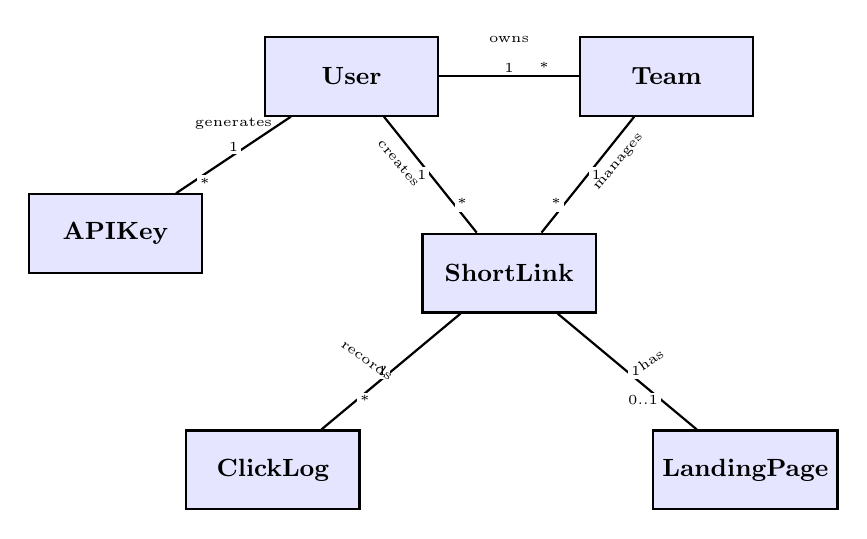
\begin{tikzpicture}[
    entity/.style={rectangle, draw=black, thick, fill=blue!10, minimum width=2.2cm, minimum height=1cm, align=center, font=\small\bfseries},
    relation/.style={diamond, draw=black, thick, fill=yellow!20, minimum width=1.2cm, minimum height=0.8cm, align=center, font=\tiny},
    edge/.style={thick},
    label/.style={font=\tiny, fill=white, inner sep=1pt}
]

% Entities
\node[entity] (user) at (0, 0) {User};
\node[entity] (team) at (4, 0) {Team};
\node[entity] (shortlink) at (2, -2.5) {ShortLink};
\node[entity] (clicklog) at (-1, -5) {ClickLog};
\node[entity] (landingpage) at (5, -5) {LandingPage};
\node[entity] (apikey) at (-3, -2) {APIKey};

% User - Team (owns)
\draw[edge] (user) -- node[label, above] {1} (team) node[label, near end, above] {*};
\node[font=\tiny, above] at (2, 0.3) {owns};

% User - ShortLink (creates)
\draw[edge] (user) -- node[label, left] {1} (shortlink) node[label, near end, right] {*};
\node[font=\tiny, rotate=-50] at (0.6, -1.1) {creates};

% User - APIKey (generates)
\draw[edge] (user) -- node[label, above] {1} (apikey) node[label, near end, below] {*};
\node[font=\tiny, above] at (-1.5, -0.8) {generates};

% Team - ShortLink (manages)
\draw[edge] (team) -- node[label, right] {1} (shortlink) node[label, near end, left] {*};
\node[font=\tiny, rotate=50] at (3.4, -1.1) {manages};

% ShortLink - ClickLog (records)
\draw[edge] (shortlink) -- node[label, left] {1} (clicklog) node[label, near end, right] {*};
\node[font=\tiny, rotate=-35] at (0.2, -3.6) {records};

% ShortLink - LandingPage (has)
\draw[edge] (shortlink) -- node[label, right] {1} (landingpage) node[label, near end, left] {0..1};
\node[font=\tiny, rotate=35] at (3.8, -3.6) {has};

\end{tikzpicture}
\caption{Entity-Relationship Diagram}
\end{figure}

\subsubsection{Entity Descriptions}

\begin{table}[H]
\centering
\begin{tabular}{|l|p{10cm}|}
\hline
\textbf{Entity} & \textbf{Description} \\
\hline
User & Stores user personal information including username, email, and Argon2 password hash \\
Team & Stores team information for collaborative link management \\
ShortLink & Core entity storing short link mappings with metadata \\
ClickLog & Records detailed analytics data with anonymized IP (SHA256) \\
LandingPage & Stores custom landing page HTML/CSS content \\
APIKey & Manages programmatic API access with hashed keys \\
\hline
\end{tabular}
\caption{Entity Descriptions}
\end{table}

\subsubsection{Database Indexing Strategy}

Database indexing balances read performance against write overhead. TinyBridge exhibits a read-heavy workload—redirects occur thousands of times per second while link creation happens infrequently—making aggressive read optimization the appropriate strategy.

The \textbf{unique index on short\_code} is the most critical index, serving every redirect request. This B-tree index enables O(log n) lookups that execute in under 1ms even with millions of records. The uniqueness constraint also enforces data integrity, preventing duplicate short codes at the database level as a fallback to the Bloom filter.

The \textbf{index on user\_id} optimizes the dashboard query that lists a user's links. Without this index, displaying a user's links would require a full table scan. With the index, the query filters directly to the relevant rows, supporting pagination through cursor-based navigation.

The \textbf{composite index on (link\_id, clicked\_at)} accelerates time-range analytics queries such as "clicks in the last 7 days." The column order matters: link\_id first enables filtering to a specific link, then clicked\_at enables efficient range scans within that subset. This index also supports ORDER BY clicked\_at queries without additional sorting.

The \textbf{composite index on (link\_id, clicked\_at, country)} extends the previous index for geographic analytics. Including country as the third column creates a covering index for country-grouped queries, avoiding heap lookups when only these three columns are needed. This optimization reduces I/O for the geographic distribution dashboard.

% ==================== Chapter 5: Software Analysis ====================
\newpage
\section{Software Analysis}

\subsection{Context Model}

The Context Model diagram illustrates TinyBridge's system boundary and its interactions with external entities and systems.

\begin{figure}[H]
\centering
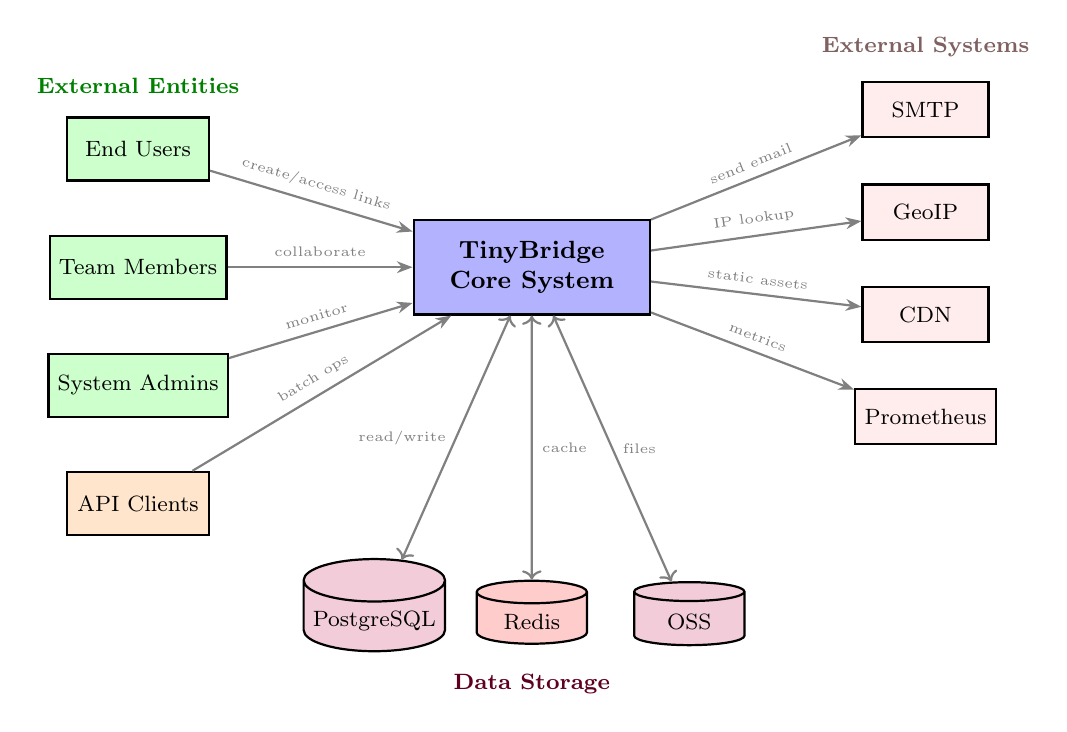
\begin{tikzpicture}[
    entity/.style={rectangle, draw=black, thick, fill=green!20, minimum width=1.8cm, minimum height=0.8cm, align=center, font=\footnotesize},
    system/.style={rectangle, draw=black, thick, fill=blue!30, minimum width=3cm, minimum height=1.2cm, align=center, font=\small\bfseries},
    external/.style={rectangle, draw=black, thick, fill=pink!30, minimum width=1.6cm, minimum height=0.7cm, align=center, font=\footnotesize},
    storage/.style={cylinder, draw=black, thick, fill=purple!20, minimum width=1.4cm, minimum height=0.8cm, align=center, font=\footnotesize, shape border rotate=90, aspect=0.3},
    arrow/.style={-{Stealth[length=2mm]}, thick, gray},
    label/.style={font=\tiny, text=gray}
]

% Central System
\node[system] (core) at (0, 0) {TinyBridge\\Core System};

% External Entities (left side)
\node[entity] (user) at (-5, 1.5) {End Users};
\node[entity] (team) at (-5, 0) {Team Members};
\node[entity] (admin) at (-5, -1.5) {System Admins};
\node[entity, fill=orange!20] (api) at (-5, -3) {API Clients};

% External Systems (right side)
\node[external] (smtp) at (5, 2) {SMTP};
\node[external] (geoip) at (5, 0.7) {GeoIP};
\node[external] (cdn) at (5, -0.6) {CDN};
\node[external] (monitor) at (5, -1.9) {Prometheus};

% Data Storage (bottom)
\node[storage] (postgres) at (-2, -4.5) {PostgreSQL};
\node[storage, fill=red!20] (redis) at (0, -4.5) {Redis};
\node[storage] (oss) at (2, -4.5) {OSS};

% Arrows from entities to system
\draw[arrow] (user) -- node[label, above, sloped] {create/access links} (core);
\draw[arrow] (team) -- node[label, above, sloped] {collaborate} (core);
\draw[arrow] (admin) -- node[label, above, sloped] {monitor} (core);
\draw[arrow] (api) -- node[label, above, sloped] {batch ops} (core);

% Arrows from system to external systems
\draw[arrow] (core) -- node[label, above, sloped] {send email} (smtp);
\draw[arrow] (core) -- node[label, above, sloped] {IP lookup} (geoip);
\draw[arrow] (core) -- node[label, above, sloped] {static assets} (cdn);
\draw[arrow] (core) -- node[label, above, sloped] {metrics} (monitor);

% Arrows from system to storage
\draw[arrow, <->] (core) -- node[label, left] {read/write} (postgres);
\draw[arrow, <->] (core) -- node[label, right] {cache} (redis);
\draw[arrow, <->] (core) -- node[label, right] {files} (oss);

% Group labels
\node[font=\footnotesize\bfseries, text=green!50!black] at (-5, 2.3) {External Entities};
\node[font=\footnotesize\bfseries, text=pink!50!black] at (5, 2.8) {External Systems};
\node[font=\footnotesize\bfseries, text=purple!50!black] at (0, -5.3) {Data Storage};

\end{tikzpicture}
\caption{Context Model Diagram}
\end{figure}

\begin{table}[H]
\centering
\begin{tabular}{|l|p{9cm}|}
\hline
\textbf{Entity} & \textbf{Interaction} \\
\hline
End Users & Register/Login, Create/Manage Short Links, View Analytics \\
Team Members & Collaborate on shared links, Manage team resources \\
System Admins & Monitor system performance, Manage user accounts \\
API Clients & Batch operations, Data import/export \\
Email Service & User verification, Password reset, Team invitations \\
GeoIP Service & IP address to geographic location mapping \\
CDN & Static asset delivery acceleration \\
Monitoring & Performance metrics collection and visualization \\
\hline
\end{tabular}
\caption{Context Model Entity Interactions}
\end{table}

\subsection{Business Process Model}

\subsubsection{Short Link Creation Process}

\begin{figure}[H]
\centering
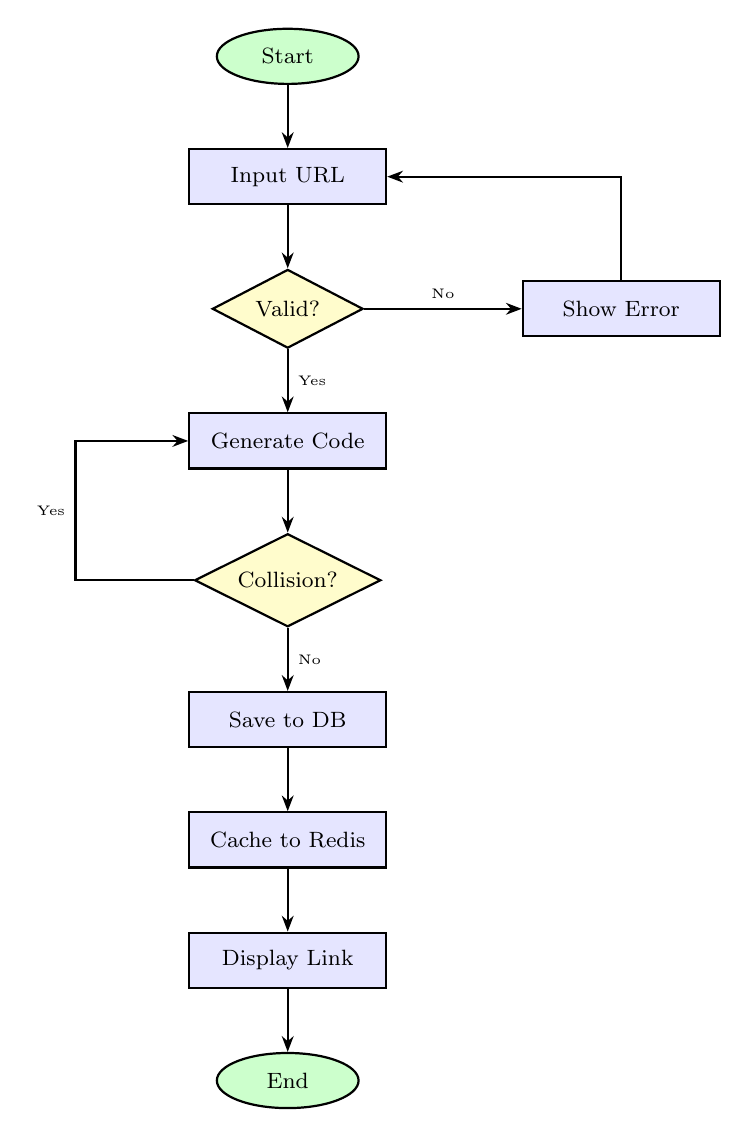
\begin{tikzpicture}[
    startstop/.style={ellipse, draw=black, thick, fill=green!20, minimum width=1.8cm, minimum height=0.7cm, align=center, font=\footnotesize},
    process/.style={rectangle, draw=black, thick, fill=blue!10, minimum width=2.5cm, minimum height=0.7cm, align=center, font=\footnotesize},
    decision/.style={diamond, draw=black, thick, fill=yellow!20, minimum width=1.8cm, minimum height=1cm, align=center, font=\footnotesize, aspect=2},
    arrow/.style={-{Stealth[length=2mm]}, thick},
    node distance=0.8cm
]

% Main flow
\node[startstop] (start) {Start};
\node[process, below=of start] (input) {Input URL};
\node[decision, below=of input] (validate) {Valid?};
\node[process, right=2cm of validate] (error) {Show Error};
\node[process, below=of validate] (generate) {Generate Code};
\node[decision, below=of generate] (collision) {Collision?};
\node[process, below=of collision] (save) {Save to DB};
\node[process, below=of save] (cache) {Cache to Redis};
\node[process, below=of cache] (display) {Display Link};
\node[startstop, below=of display] (end) {End};

% Arrows
\draw[arrow] (start) -- (input);
\draw[arrow] (input) -- (validate);
\draw[arrow] (validate) -- node[above, font=\tiny] {No} (error);
\draw[arrow] (error) |- (input);
\draw[arrow] (validate) -- node[right, font=\tiny] {Yes} (generate);
\draw[arrow] (generate) -- (collision);
\draw[arrow] (collision.west) -- ++(-1.5,0) |- node[left, font=\tiny, pos=0.25] {Yes} (generate.west);
\draw[arrow] (collision) -- node[right, font=\tiny] {No} (save);
\draw[arrow] (save) -- (cache);
\draw[arrow] (cache) -- (display);
\draw[arrow] (display) -- (end);

\end{tikzpicture}
\caption{Short Link Creation Process Flow}
\end{figure}

\subsubsection{Process Description}

\begin{enumerate}
    \item \textbf{URL Input}: User enters the original URL to be shortened
    \item \textbf{Validation}: System validates URL format (HTTP/HTTPS protocol)
    \item \textbf{Code Generation}:
    \begin{itemize}
        \item Random: Base62 algorithm generates 6-8 character code
        \item Custom: User specifies desired code
    \end{itemize}
    \item \textbf{Collision Detection}:
    \begin{itemize}
        \item Bloom Filter provides O(1) preliminary check
        \item Database confirms if potential collision exists
    \end{itemize}
    \item \textbf{Storage}: Link mapping saved to PostgreSQL, cached in Redis
    \item \textbf{Configuration}: Optional expiration and custom domain settings
    \item \textbf{Result}: Short link displayed with copy/QR/landing page options
\end{enumerate}

\subsubsection{User Registration and Login Process}

\begin{figure}[H]
\centering
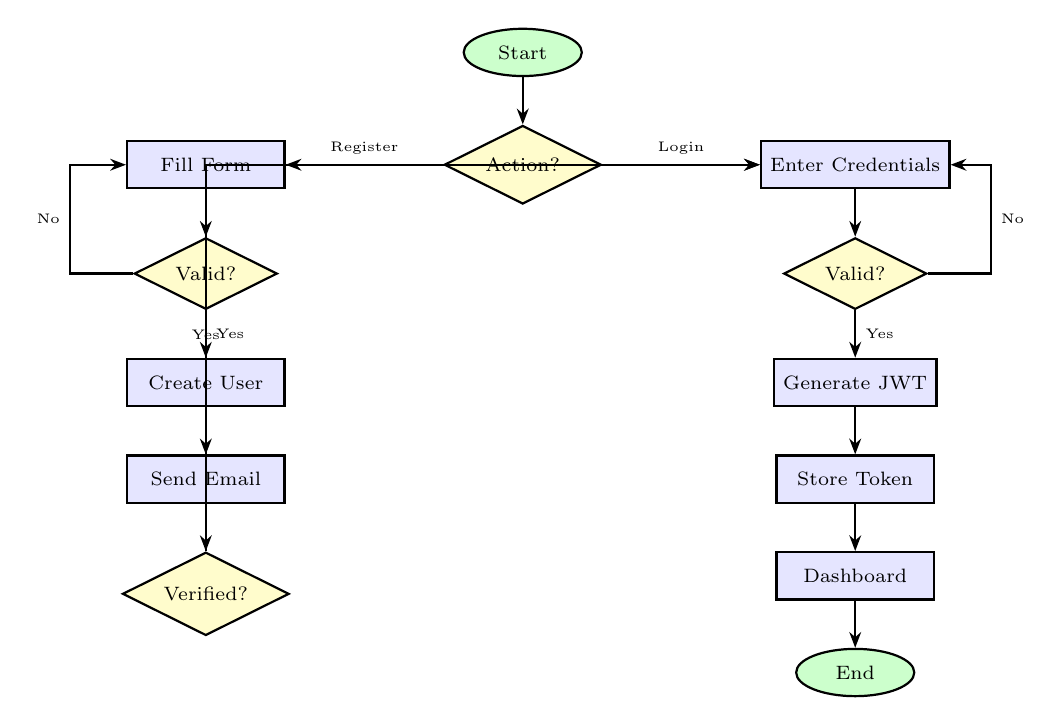
\begin{tikzpicture}[
    startstop/.style={ellipse, draw=black, thick, fill=green!20, minimum width=1.5cm, minimum height=0.6cm, align=center, font=\scriptsize},
    process/.style={rectangle, draw=black, thick, fill=blue!10, minimum width=2cm, minimum height=0.6cm, align=center, font=\scriptsize},
    decision/.style={diamond, draw=black, thick, fill=yellow!20, minimum width=1.5cm, minimum height=0.8cm, align=center, font=\scriptsize, aspect=2},
    arrow/.style={-{Stealth[length=2mm]}, thick},
    node distance=0.6cm
]

% Main flow
\node[startstop] (start) {Start};
\node[decision, below=of start] (choice) {Action?};

% Register branch
\node[process, left=2cm of choice] (regform) {Fill Form};
\node[decision, below=of regform] (regvalid) {Valid?};
\node[process, below=of regvalid] (createuser) {Create User};
\node[process, below=of createuser] (sendemail) {Send Email};
\node[decision, below=of sendemail] (verify) {Verified?};

% Login branch
\node[process, right=2cm of choice] (loginform) {Enter Credentials};
\node[decision, below=of loginform] (loginvalid) {Valid?};
\node[process, below=of loginvalid] (gentoken) {Generate JWT};
\node[process, below=of gentoken] (store) {Store Token};
\node[process, below=of store] (dashboard) {Dashboard};
\node[startstop, below=of dashboard] (end) {End};

% Arrows - Choice
\draw[arrow] (start) -- (choice);
\draw[arrow] (choice) -- node[above, font=\tiny] {Register} (regform);
\draw[arrow] (choice) -- node[above, font=\tiny] {Login} (loginform);

% Register flow
\draw[arrow] (regform) -- (regvalid);
\draw[arrow] (regvalid.west) -- ++(-0.8,0) |- node[left, font=\tiny, pos=0.25] {No} (regform.west);
\draw[arrow] (regvalid) -- node[right, font=\tiny] {Yes} (createuser);
\draw[arrow] (createuser) -- (sendemail);
\draw[arrow] (sendemail) -- (verify);
\draw[arrow] (verify) |- node[below, font=\tiny, pos=0.3] {Yes} (loginform);

% Login flow
\draw[arrow] (loginform) -- (loginvalid);
\draw[arrow] (loginvalid.east) -- ++(0.8,0) |- node[right, font=\tiny, pos=0.25] {No} (loginform.east);
\draw[arrow] (loginvalid) -- node[right, font=\tiny] {Yes} (gentoken);
\draw[arrow] (gentoken) -- (store);
\draw[arrow] (store) -- (dashboard);
\draw[arrow] (dashboard) -- (end);

\end{tikzpicture}
\caption{User Registration and Login Process Flow}
\end{figure}

The registration process validates user input (email format, password strength), creates a user record with Argon2-hashed password, and sends a verification email. Upon email verification, users can login with their credentials, receive a JWT token (valid for 7 days), and access the dashboard.

\subsubsection{QR Code Generation Process}

\begin{figure}[H]
\centering
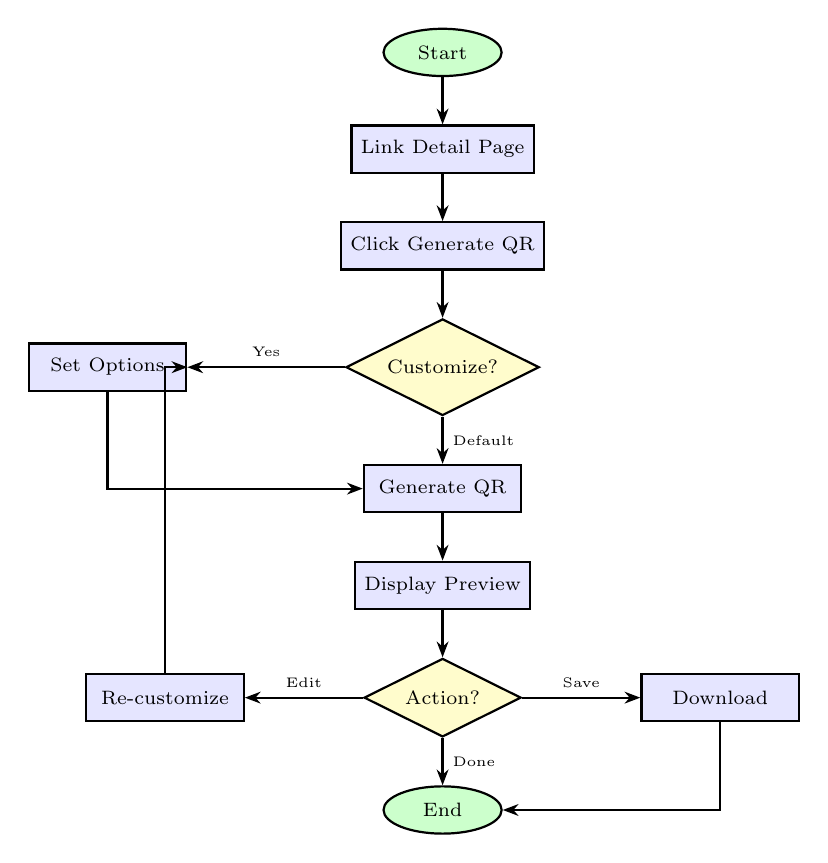
\begin{tikzpicture}[
    startstop/.style={ellipse, draw=black, thick, fill=green!20, minimum width=1.5cm, minimum height=0.6cm, align=center, font=\scriptsize},
    process/.style={rectangle, draw=black, thick, fill=blue!10, minimum width=2cm, minimum height=0.6cm, align=center, font=\scriptsize},
    decision/.style={diamond, draw=black, thick, fill=yellow!20, minimum width=1.5cm, minimum height=0.8cm, align=center, font=\scriptsize, aspect=2},
    arrow/.style={-{Stealth[length=2mm]}, thick},
    node distance=0.6cm
]

\node[startstop] (start) {Start};
\node[process, below=of start] (linkpage) {Link Detail Page};
\node[process, below=of linkpage] (clickqr) {Click Generate QR};
\node[decision, below=of clickqr] (customize) {Customize?};

\node[process, left=2cm of customize] (custom) {Set Options};
\node[process, below=of customize] (generate) {Generate QR};
\node[process, below=of generate] (preview) {Display Preview};
\node[decision, below=of preview] (action) {Action?};

\node[process, left=1.5cm of action] (recustom) {Re-customize};
\node[process, right=1.5cm of action] (download) {Download};
\node[startstop, below=of action] (end) {End};

% Arrows
\draw[arrow] (start) -- (linkpage);
\draw[arrow] (linkpage) -- (clickqr);
\draw[arrow] (clickqr) -- (customize);
\draw[arrow] (customize) -- node[above, font=\tiny] {Yes} (custom);
\draw[arrow] (custom) |- (generate);
\draw[arrow] (customize) -- node[right, font=\tiny] {Default} (generate);
\draw[arrow] (generate) -- (preview);
\draw[arrow] (preview) -- (action);
\draw[arrow] (action) -- node[above, font=\tiny] {Edit} (recustom);
\draw[arrow] (recustom) |- (custom);
\draw[arrow] (action) -- node[above, font=\tiny] {Save} (download);
\draw[arrow] (download) |- (end);
\draw[arrow] (action) -- node[right, font=\tiny] {Done} (end);

\end{tikzpicture}
\caption{QR Code Generation Process Flow}
\end{figure}

QR code generation is performed entirely on the client-side using the qrcode.js library, requiring no backend requests. Users can customize color, size (128/256/512px), and error correction level (L/M/Q/H). The generated QR code encodes the short URL, ensuring it remains valid even if the target URL changes.

\subsubsection{Analytics Processing}

\begin{figure}[H]
\centering
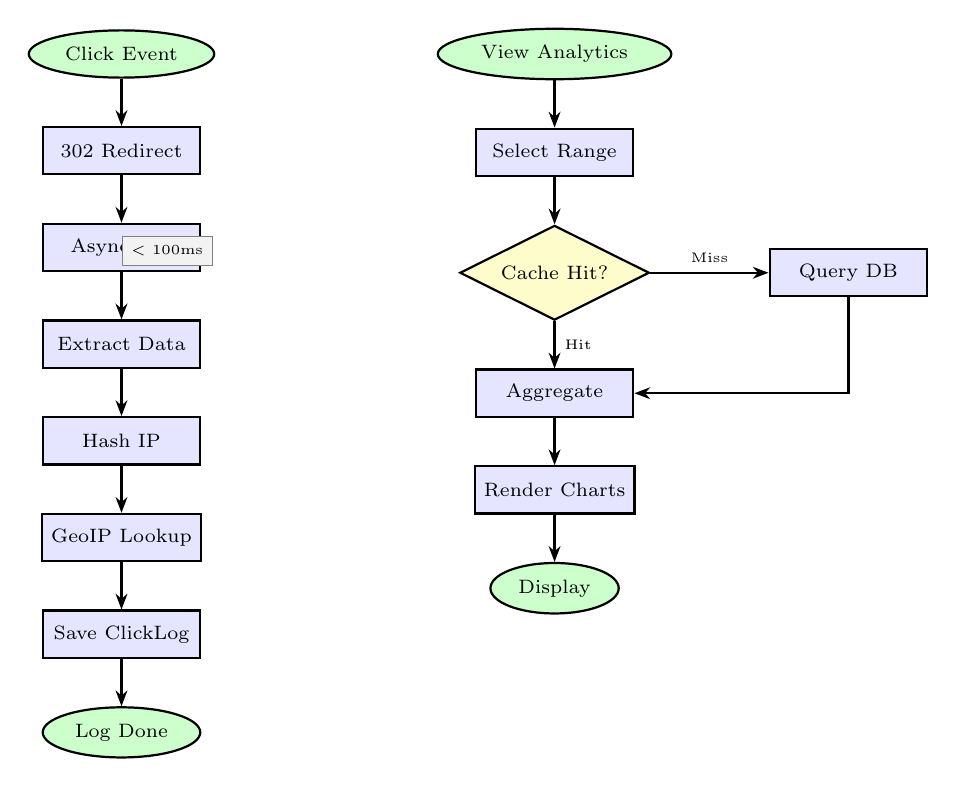
\begin{tikzpicture}[
    startstop/.style={ellipse, draw=black, thick, fill=green!20, minimum width=1.5cm, minimum height=0.6cm, align=center, font=\scriptsize},
    process/.style={rectangle, draw=black, thick, fill=blue!10, minimum width=2cm, minimum height=0.6cm, align=center, font=\scriptsize},
    decision/.style={diamond, draw=black, thick, fill=yellow!20, minimum width=1.5cm, minimum height=0.8cm, align=center, font=\scriptsize, aspect=2},
    arrow/.style={-{Stealth[length=2mm]}, thick},
    note/.style={rectangle, draw=gray, fill=gray!10, font=\tiny, align=left},
    node distance=0.6cm
]

% Click logging flow (left)
\node[startstop] (start1) at (0, 0) {Click Event};
\node[process, below=of start1] (redirect) {302 Redirect};
\node[process, below=of redirect] (async) {Async Log};
\node[process, below=of async] (extract) {Extract Data};
\node[process, below=of extract] (haship) {Hash IP};
\node[process, below=of haship] (geoip) {GeoIP Lookup};
\node[process, below=of geoip] (savelog) {Save ClickLog};
\node[startstop, below=of savelog] (end1) {Log Done};

% Analytics view flow (right)
\node[startstop] (start2) at (5.5, 0) {View Analytics};
\node[process, below=of start2] (select) {Select Range};
\node[decision, below=of select] (cache) {Cache Hit?};
\node[process, right=1.5cm of cache] (query) {Query DB};
\node[process, below=of cache] (aggregate) {Aggregate};
\node[process, below=of aggregate] (charts) {Render Charts};
\node[startstop, below=of charts] (end2) {Display};

% Arrows - Click flow
\draw[arrow] (start1) -- (redirect);
\draw[arrow] (redirect) -- (async);
\draw[arrow] (async) -- (extract);
\draw[arrow] (extract) -- (haship);
\draw[arrow] (haship) -- (geoip);
\draw[arrow] (geoip) -- (savelog);
\draw[arrow] (savelog) -- (end1);

% Arrows - Analytics flow
\draw[arrow] (start2) -- (select);
\draw[arrow] (select) -- (cache);
\draw[arrow] (cache) -- node[above, font=\tiny] {Miss} (query);
\draw[arrow] (query) |- (aggregate);
\draw[arrow] (cache) -- node[right, font=\tiny] {Hit} (aggregate);
\draw[arrow] (aggregate) -- (charts);
\draw[arrow] (charts) -- (end2);

% Notes
\node[note] at (0, -2.5) [right] {< 100ms};

\end{tikzpicture}
\caption{Analytics Processing Flow (Click Logging and Data Visualization)}
\end{figure}

Click events are logged asynchronously to avoid blocking redirects. IP addresses are hashed with SHA256 and daily-rotating salt for privacy compliance (GDPR/CCPA). Analytics queries use Redis caching (1-hour TTL) to reduce database load. The system renders multiple chart types: line charts for time trends, pie charts for device distribution, and geographic maps.

\subsubsection{Landing Page Editor Process}

\begin{figure}[H]
\centering
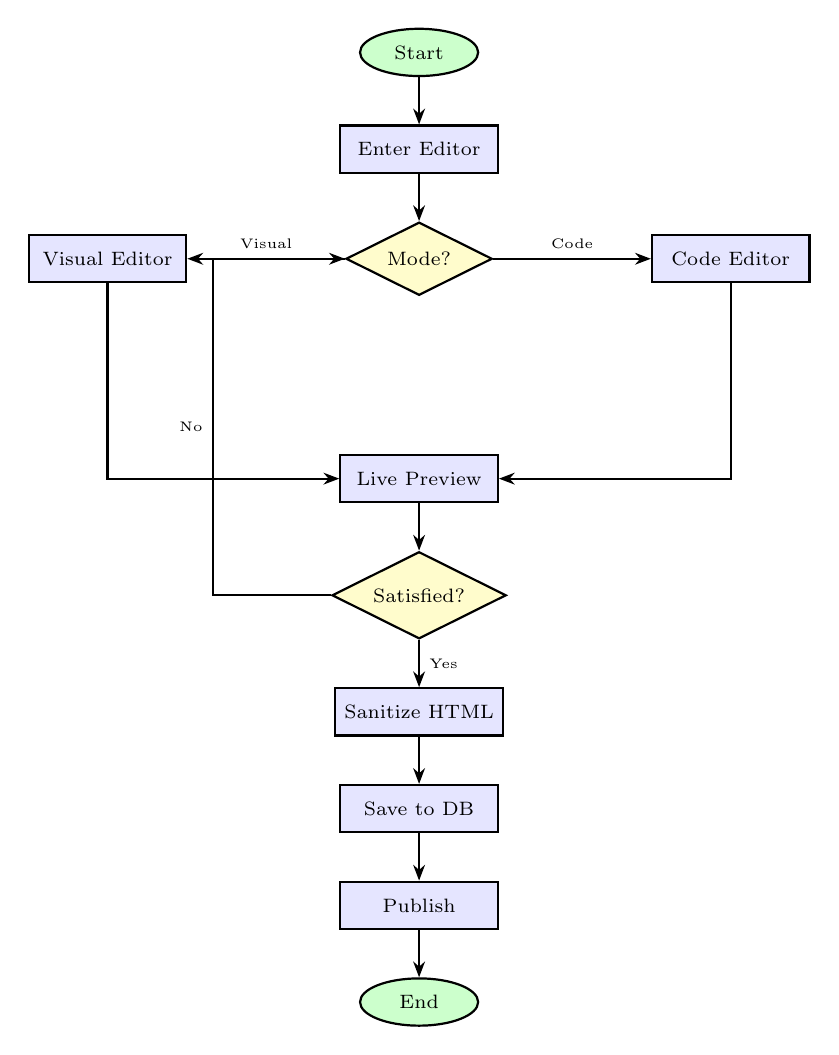
\begin{tikzpicture}[
    startstop/.style={ellipse, draw=black, thick, fill=green!20, minimum width=1.5cm, minimum height=0.6cm, align=center, font=\scriptsize},
    process/.style={rectangle, draw=black, thick, fill=blue!10, minimum width=2cm, minimum height=0.6cm, align=center, font=\scriptsize},
    decision/.style={diamond, draw=black, thick, fill=yellow!20, minimum width=1.5cm, minimum height=0.8cm, align=center, font=\scriptsize, aspect=2},
    arrow/.style={-{Stealth[length=2mm]}, thick},
    node distance=0.6cm
]

\node[startstop] (start) {Start};
\node[process, below=of start] (enter) {Enter Editor};
\node[decision, below=of enter] (mode) {Mode?};

\node[process, left=2cm of mode] (visual) {Visual Editor};
\node[process, right=2cm of mode] (code) {Code Editor};

\node[process, below=2cm of mode] (preview) {Live Preview};
\node[decision, below=of preview] (satisfied) {Satisfied?};
\node[process, below=of satisfied] (sanitize) {Sanitize HTML};
\node[process, below=of sanitize] (save) {Save to DB};
\node[process, below=of save] (publish) {Publish};
\node[startstop, below=of publish] (end) {End};

% Arrows
\draw[arrow] (start) -- (enter);
\draw[arrow] (enter) -- (mode);
\draw[arrow] (mode) -- node[above, font=\tiny] {Visual} (visual);
\draw[arrow] (mode) -- node[above, font=\tiny] {Code} (code);
\draw[arrow] (visual) |- (preview);
\draw[arrow] (code) |- (preview);
\draw[arrow] (preview) -- (satisfied);
\draw[arrow] (satisfied.west) -- ++(-1.5,0) |- node[left, font=\tiny, pos=0.25] {No} (mode.west);
\draw[arrow] (satisfied) -- node[right, font=\tiny] {Yes} (sanitize);
\draw[arrow] (sanitize) -- (save);
\draw[arrow] (save) -- (publish);
\draw[arrow] (publish) -- (end);

\end{tikzpicture}
\caption{Landing Page Editor Process Flow}
\end{figure}

The landing page editor supports two modes: a visual drag-and-drop editor for non-technical users and a code editor (Monaco Editor) for developers. All HTML content is sanitized using DOMPurify before storage to prevent XSS attacks. Live preview allows real-time feedback during editing.

\subsubsection{Batch API Operations}

\begin{figure}[H]
\centering
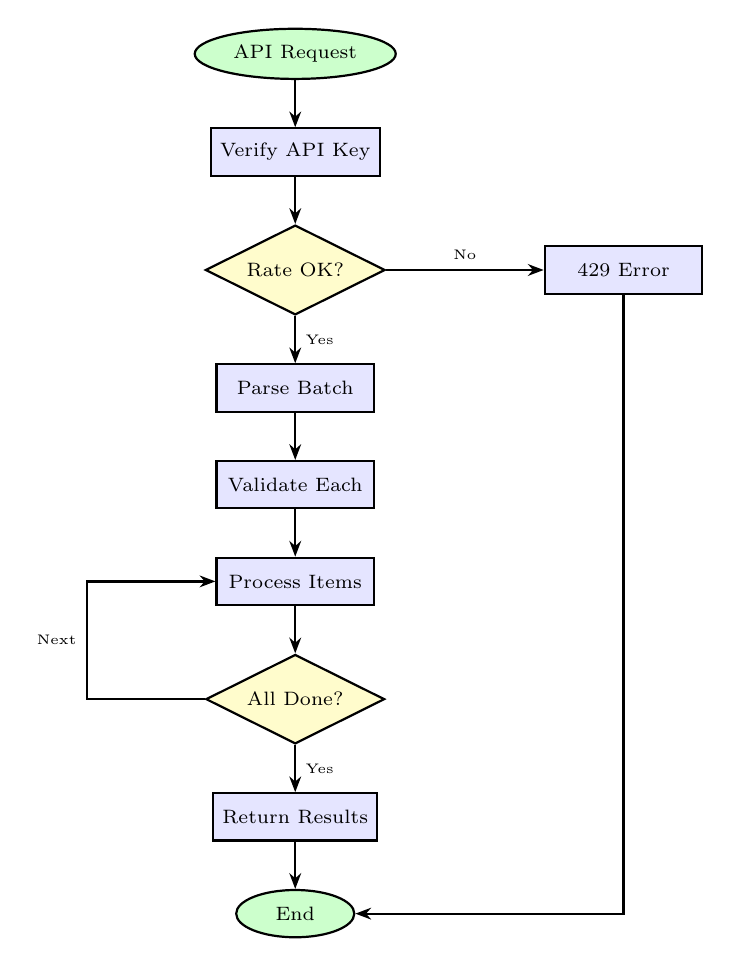
\begin{tikzpicture}[
    startstop/.style={ellipse, draw=black, thick, fill=green!20, minimum width=1.5cm, minimum height=0.6cm, align=center, font=\scriptsize},
    process/.style={rectangle, draw=black, thick, fill=blue!10, minimum width=2cm, minimum height=0.6cm, align=center, font=\scriptsize},
    decision/.style={diamond, draw=black, thick, fill=yellow!20, minimum width=1.5cm, minimum height=0.8cm, align=center, font=\scriptsize, aspect=2},
    arrow/.style={-{Stealth[length=2mm]}, thick},
    node distance=0.6cm
]

\node[startstop] (start) {API Request};
\node[process, below=of start] (auth) {Verify API Key};
\node[decision, below=of auth] (ratelimit) {Rate OK?};
\node[process, right=2cm of ratelimit] (reject) {429 Error};

\node[process, below=of ratelimit] (parse) {Parse Batch};
\node[process, below=of parse] (validate) {Validate Each};
\node[process, below=of validate] (process) {Process Items};
\node[decision, below=of process] (complete) {All Done?};
\node[process, below=of complete] (response) {Return Results};
\node[startstop, below=of response] (end) {End};

% Arrows
\draw[arrow] (start) -- (auth);
\draw[arrow] (auth) -- (ratelimit);
\draw[arrow] (ratelimit) -- node[above, font=\tiny] {No} (reject);
\draw[arrow] (reject) |- (end);
\draw[arrow] (ratelimit) -- node[right, font=\tiny] {Yes} (parse);
\draw[arrow] (parse) -- (validate);
\draw[arrow] (validate) -- (process);
\draw[arrow] (process) -- (complete);
\draw[arrow] (complete.west) -- ++(-1.5,0) |- node[left, font=\tiny, pos=0.25] {Next} (process.west);
\draw[arrow] (complete) -- node[right, font=\tiny] {Yes} (response);
\draw[arrow] (response) -- (end);

\end{tikzpicture}
\caption{Batch API Operations Process Flow}
\end{figure}

The batch API supports bulk creation, update, and deletion of short links. API authentication uses API keys with rate limiting (1000 requests/hour for API clients). Each item in the batch is validated individually, and the response includes success/failure status for each operation, enabling partial success handling.

\subsection{Class Diagram}

\begin{figure}[H]
\centering
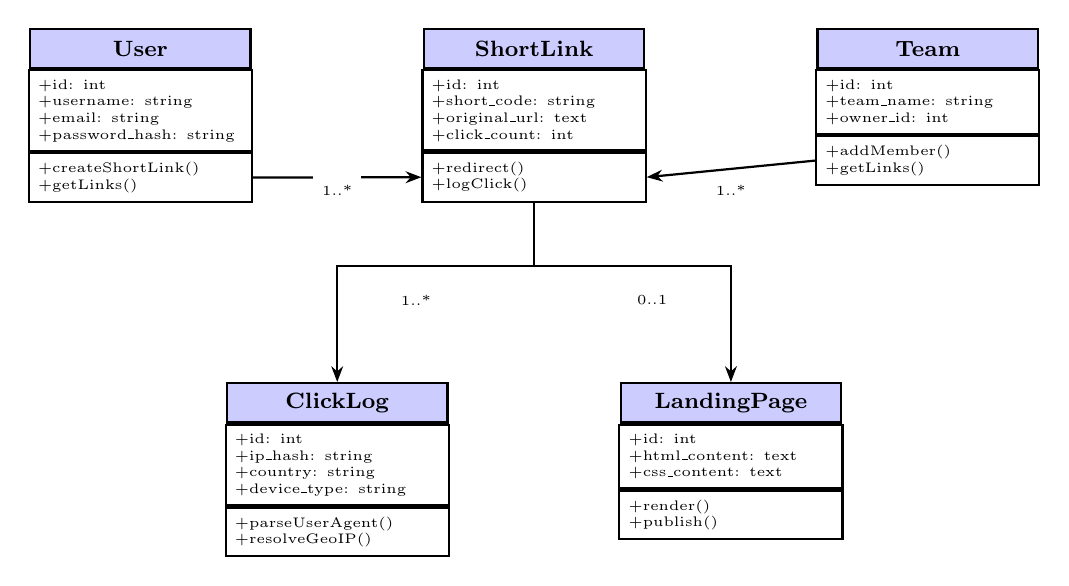
\begin{tikzpicture}[
    class/.style={rectangle, draw=black, thick, fill=white, minimum width=2.8cm, align=left, font=\tiny, text width=2.6cm},
    classname/.style={rectangle, draw=black, thick, fill=blue!20, minimum width=2.8cm, minimum height=0.5cm, align=center, font=\footnotesize\bfseries},
    arrow/.style={-{Stealth[length=2mm]}, thick},
    node distance=0.3cm
]

% User class
\node[classname] (username) at (0, 0) {User};
\node[class, below=0pt of username] (userattr) {+id: int\\+username: string\\+email: string\\+password\_hash: string};
\node[class, below=0pt of userattr] (usermeth) {+createShortLink()\\+getLinks()};

% ShortLink class
\node[classname] (linkname) at (5, 0) {ShortLink};
\node[class, below=0pt of linkname] (linkattr) {+id: int\\+short\_code: string\\+original\_url: text\\+click\_count: int};
\node[class, below=0pt of linkattr] (linkmeth) {+redirect()\\+logClick()};

% Team class
\node[classname] (teamname) at (10, 0) {Team};
\node[class, below=0pt of teamname] (teamattr) {+id: int\\+team\_name: string\\+owner\_id: int};
\node[class, below=0pt of teamattr] (teammeth) {+addMember()\\+getLinks()};

% ClickLog class
\node[classname] (logname) at (2.5, -4.5) {ClickLog};
\node[class, below=0pt of logname] (logattr) {+id: int\\+ip\_hash: string\\+country: string\\+device\_type: string};
\node[class, below=0pt of logattr] (logmeth) {+parseUserAgent()\\+resolveGeoIP()};

% LandingPage class
\node[classname] (lpname) at (7.5, -4.5) {LandingPage};
\node[class, below=0pt of lpname] (lpattr) {+id: int\\+html\_content: text\\+css\_content: text};
\node[class, below=0pt of lpattr] (lpmeth) {+render()\\+publish()};

% Relationships - 用线连接,标注放在线的中间偏上
\draw[arrow] (usermeth.east) -- (linkmeth.west);
\node[font=\tiny, fill=white] at (2.5, -1.8) {1..*};

\draw[arrow] (teammeth.west) -- (linkmeth.east);
\node[font=\tiny, fill=white] at (7.5, -1.8) {1..*};

\draw[arrow] (linkmeth.south) -- ++(0, -0.8) -| (logname.north);
\node[font=\tiny, fill=white] at (3.5, -3.2) {1..*};

\draw[arrow] (linkmeth.south) -- ++(0, -0.8) -| (lpname.north);
\node[font=\tiny, fill=white] at (6.5, -3.2) {0..1};

\end{tikzpicture}
\caption{Class Diagram}
\end{figure}

\subsection{Sequence Diagrams}

\subsubsection{Short Link Creation Sequence}

\begin{figure}[H]
\centering
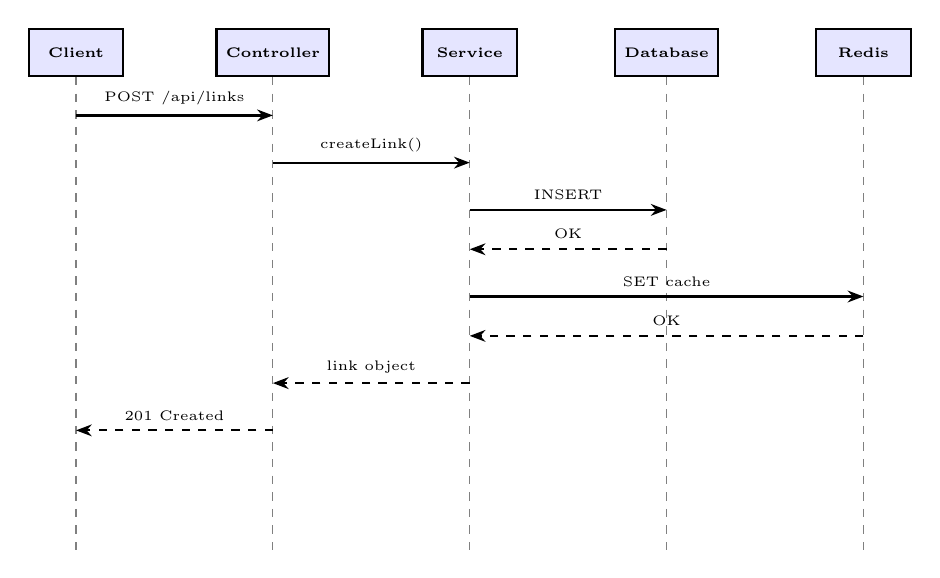
\begin{tikzpicture}[
    actor/.style={rectangle, draw=black, thick, fill=blue!10, minimum width=1.2cm, minimum height=0.6cm, align=center, font=\tiny\bfseries},
    arrow/.style={-{Stealth[length=2mm]}, thick},
    msg/.style={font=\tiny},
    lifeline/.style={dashed, gray}
]

% Actors
\node[actor] (client) at (0, 0) {Client};
\node[actor] (controller) at (2.5, 0) {Controller};
\node[actor] (service) at (5, 0) {Service};
\node[actor] (db) at (7.5, 0) {Database};
\node[actor] (redis) at (10, 0) {Redis};

% Lifelines
\draw[lifeline] (client.south) -- ++(0, -6);
\draw[lifeline] (controller.south) -- ++(0, -6);
\draw[lifeline] (service.south) -- ++(0, -6);
\draw[lifeline] (db.south) -- ++(0, -6);
\draw[lifeline] (redis.south) -- ++(0, -6);

% Messages
\draw[arrow] (0, -0.8) -- node[msg, above] {POST /api/links} (2.5, -0.8);
\draw[arrow] (2.5, -1.4) -- node[msg, above] {createLink()} (5, -1.4);
\draw[arrow] (5, -2.0) -- node[msg, above] {INSERT} (7.5, -2.0);
\draw[arrow, dashed] (7.5, -2.5) -- node[msg, above] {OK} (5, -2.5);
\draw[arrow] (5, -3.1) -- node[msg, above] {SET cache} (10, -3.1);
\draw[arrow, dashed] (10, -3.6) -- node[msg, above] {OK} (5, -3.6);
\draw[arrow, dashed] (5, -4.2) -- node[msg, above] {link object} (2.5, -4.2);
\draw[arrow, dashed] (2.5, -4.8) -- node[msg, above] {201 Created} (0, -4.8);

\end{tikzpicture}
\caption{Short Link Creation Sequence Diagram}
\end{figure}

\subsubsection{URL Redirect Sequence}

\begin{figure}[H]
\centering
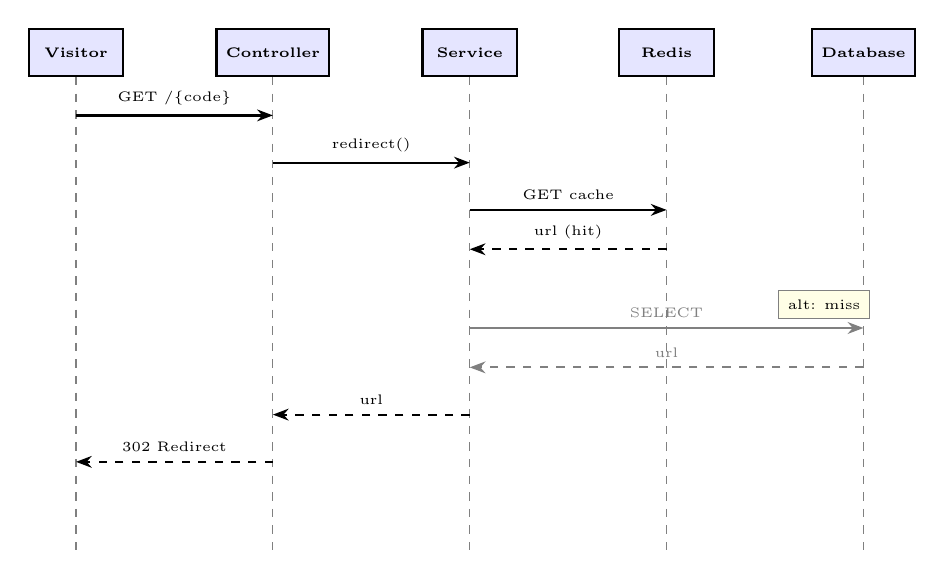
\begin{tikzpicture}[
    actor/.style={rectangle, draw=black, thick, fill=blue!10, minimum width=1.2cm, minimum height=0.6cm, align=center, font=\tiny\bfseries},
    arrow/.style={-{Stealth[length=2mm]}, thick},
    msg/.style={font=\tiny},
    lifeline/.style={dashed, gray},
    note/.style={rectangle, draw=gray, fill=yellow!10, font=\tiny, align=left}
]

% Actors
\node[actor] (visitor) at (0, 0) {Visitor};
\node[actor] (controller) at (2.5, 0) {Controller};
\node[actor] (service) at (5, 0) {Service};
\node[actor] (redis) at (7.5, 0) {Redis};
\node[actor] (db) at (10, 0) {Database};

% Lifelines
\draw[lifeline] (visitor.south) -- ++(0, -6);
\draw[lifeline] (controller.south) -- ++(0, -6);
\draw[lifeline] (service.south) -- ++(0, -6);
\draw[lifeline] (redis.south) -- ++(0, -6);
\draw[lifeline] (db.south) -- ++(0, -6);

% Messages
\draw[arrow] (0, -0.8) -- node[msg, above] {GET /\{code\}} (2.5, -0.8);
\draw[arrow] (2.5, -1.4) -- node[msg, above] {redirect()} (5, -1.4);
\draw[arrow] (5, -2.0) -- node[msg, above] {GET cache} (7.5, -2.0);
\draw[arrow, dashed] (7.5, -2.5) -- node[msg, above] {url (hit)} (5, -2.5);

% Alt: cache miss
\node[note] at (9.5, -3.2) {alt: miss};
\draw[arrow, gray] (5, -3.5) -- node[msg, above, text=gray] {SELECT} (10, -3.5);
\draw[arrow, dashed, gray] (10, -4.0) -- node[msg, above, text=gray] {url} (5, -4.0);

% Return
\draw[arrow, dashed] (5, -4.6) -- node[msg, above] {url} (2.5, -4.6);
\draw[arrow, dashed] (2.5, -5.2) -- node[msg, above] {302 Redirect} (0, -5.2);

\end{tikzpicture}
\caption{URL Redirect Sequence Diagram}
\end{figure}

\subsubsection{User Authentication Sequence}

\begin{figure}[H]
\centering
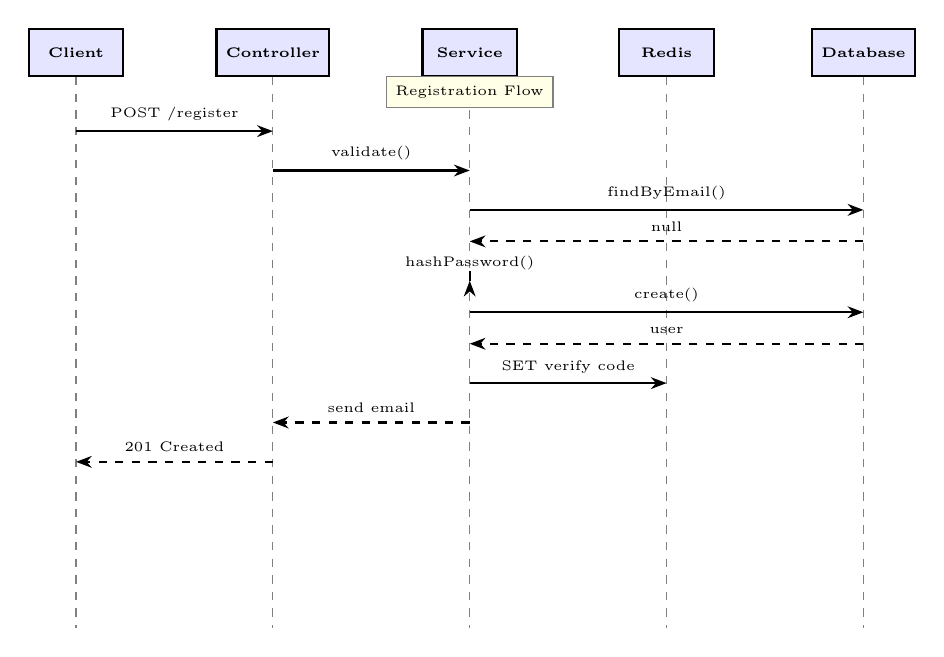
\begin{tikzpicture}[
    actor/.style={rectangle, draw=black, thick, fill=blue!10, minimum width=1.2cm, minimum height=0.6cm, align=center, font=\tiny\bfseries},
    arrow/.style={-{Stealth[length=2mm]}, thick},
    msg/.style={font=\tiny},
    lifeline/.style={dashed, gray},
    note/.style={rectangle, draw=gray, fill=yellow!10, font=\tiny, align=center}
]

% Actors
\node[actor] (client) at (0, 0) {Client};
\node[actor] (controller) at (2.5, 0) {Controller};
\node[actor] (service) at (5, 0) {Service};
\node[actor] (redis) at (7.5, 0) {Redis};
\node[actor] (db) at (10, 0) {Database};

% Lifelines
\draw[lifeline] (client.south) -- ++(0, -7);
\draw[lifeline] (controller.south) -- ++(0, -7);
\draw[lifeline] (service.south) -- ++(0, -7);
\draw[lifeline] (redis.south) -- ++(0, -7);
\draw[lifeline] (db.south) -- ++(0, -7);

% Note
\node[note] at (5, -0.5) {Registration Flow};

% Registration Messages
\draw[arrow] (0, -1) -- node[msg, above] {POST /register} (2.5, -1);
\draw[arrow] (2.5, -1.5) -- node[msg, above] {validate()} (5, -1.5);
\draw[arrow] (5, -2) -- node[msg, above] {findByEmail()} (10, -2);
\draw[arrow, dashed] (10, -2.4) -- node[msg, above] {null} (5, -2.4);
\draw[arrow] (5, -2.9) -- node[msg, above] {hashPassword()} (5, -2.9);
\draw[arrow] (5, -3.3) -- node[msg, above] {create()} (10, -3.3);
\draw[arrow, dashed] (10, -3.7) -- node[msg, above] {user} (5, -3.7);
\draw[arrow] (5, -4.2) -- node[msg, above] {SET verify code} (7.5, -4.2);
\draw[arrow, dashed] (5, -4.7) -- node[msg, above] {send email} (2.5, -4.7);
\draw[arrow, dashed] (2.5, -5.2) -- node[msg, above] {201 Created} (0, -5.2);

\end{tikzpicture}
\caption{User Authentication Sequence Diagram}
\end{figure}

The authentication flow includes input validation (email format, password strength with Zod), uniqueness checks for email and username, password hashing with Argon2, and email verification using time-limited codes stored in Redis. Login generates a JWT token valid for 7 days.

\subsubsection{Analytics Module Sequence}

\begin{figure}[H]
\centering
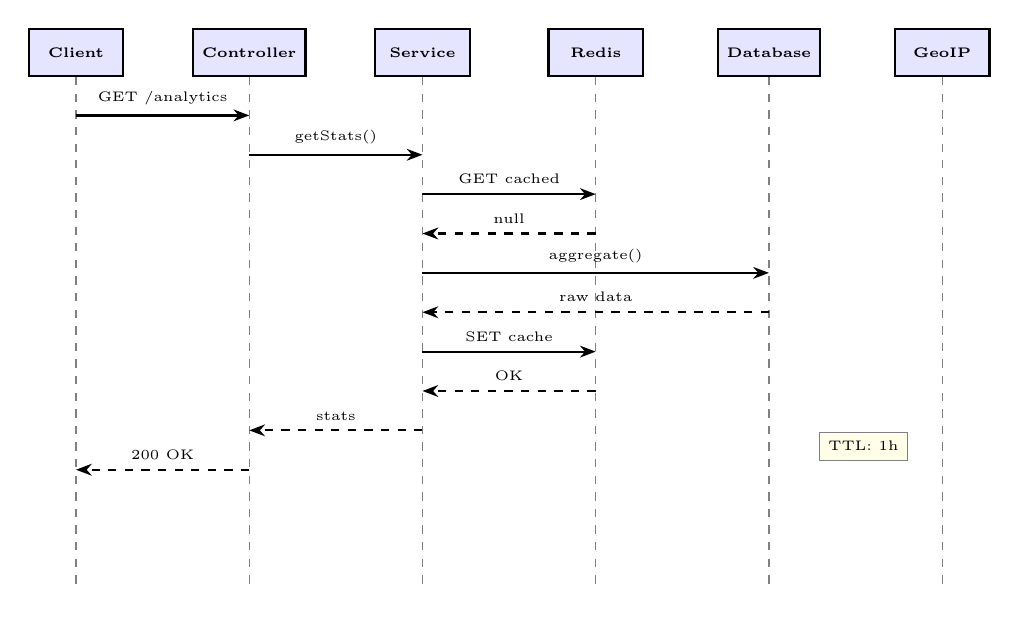
\begin{tikzpicture}[
    actor/.style={rectangle, draw=black, thick, fill=blue!10, minimum width=1.2cm, minimum height=0.6cm, align=center, font=\tiny\bfseries},
    arrow/.style={-{Stealth[length=2mm]}, thick},
    msg/.style={font=\tiny},
    lifeline/.style={dashed, gray},
    note/.style={rectangle, draw=gray, fill=yellow!10, font=\tiny, align=left}
]

% Actors
\node[actor] (client) at (0, 0) {Client};
\node[actor] (controller) at (2.2, 0) {Controller};
\node[actor] (service) at (4.4, 0) {Service};
\node[actor] (redis) at (6.6, 0) {Redis};
\node[actor] (db) at (8.8, 0) {Database};
\node[actor] (geoip) at (11, 0) {GeoIP};

% Lifelines
\draw[lifeline] (client.south) -- ++(0, -6.5);
\draw[lifeline] (controller.south) -- ++(0, -6.5);
\draw[lifeline] (service.south) -- ++(0, -6.5);
\draw[lifeline] (redis.south) -- ++(0, -6.5);
\draw[lifeline] (db.south) -- ++(0, -6.5);
\draw[lifeline] (geoip.south) -- ++(0, -6.5);

% Messages
\draw[arrow] (0, -0.8) -- node[msg, above] {GET /analytics} (2.2, -0.8);
\draw[arrow] (2.2, -1.3) -- node[msg, above] {getStats()} (4.4, -1.3);
\draw[arrow] (4.4, -1.8) -- node[msg, above] {GET cached} (6.6, -1.8);
\draw[arrow, dashed] (6.6, -2.3) -- node[msg, above] {null} (4.4, -2.3);

% DB query
\draw[arrow] (4.4, -2.8) -- node[msg, above] {aggregate()} (8.8, -2.8);
\draw[arrow, dashed] (8.8, -3.3) -- node[msg, above] {raw data} (4.4, -3.3);

% Process and cache
\draw[arrow] (4.4, -3.8) -- node[msg, above] {SET cache} (6.6, -3.8);
\draw[arrow, dashed] (6.6, -4.3) -- node[msg, above] {OK} (4.4, -4.3);

% Return
\draw[arrow, dashed] (4.4, -4.8) -- node[msg, above] {stats} (2.2, -4.8);
\draw[arrow, dashed] (2.2, -5.3) -- node[msg, above] {200 OK} (0, -5.3);

% Note
\node[note] at (10, -5) {TTL: 1h};

\end{tikzpicture}
\caption{Analytics Module Sequence Diagram}
\end{figure}

Analytics queries first check Redis cache (TTL: 1 hour). On cache miss, the system aggregates data from click\_logs table by time, geography, device, and referrer. Results are cached before returning. The system supports exports in CSV and JSON formats.

\subsubsection{Team Collaboration Sequence}

\begin{figure}[H]
\centering
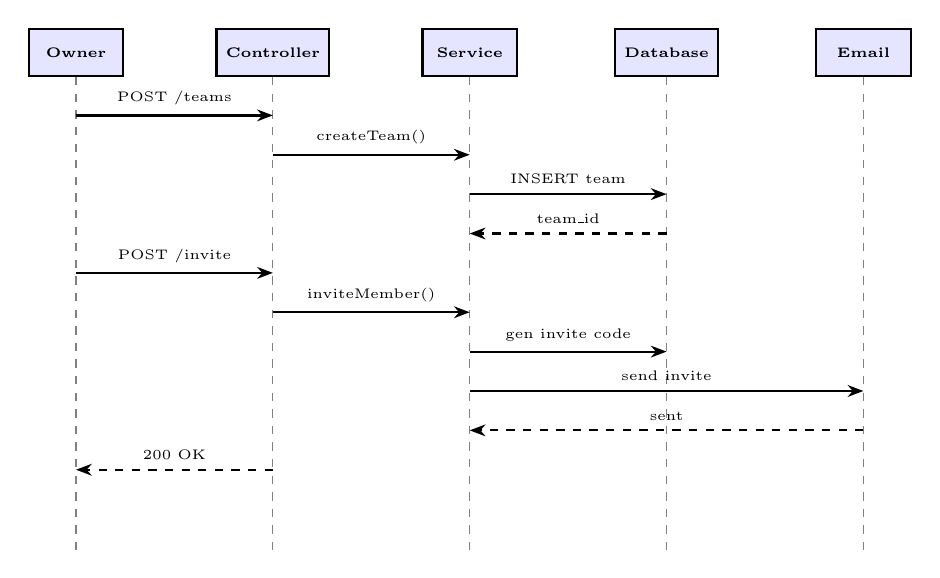
\begin{tikzpicture}[
    actor/.style={rectangle, draw=black, thick, fill=blue!10, minimum width=1.2cm, minimum height=0.6cm, align=center, font=\tiny\bfseries},
    arrow/.style={-{Stealth[length=2mm]}, thick},
    msg/.style={font=\tiny},
    lifeline/.style={dashed, gray}
]

% Actors
\node[actor] (owner) at (0, 0) {Owner};
\node[actor] (controller) at (2.5, 0) {Controller};
\node[actor] (service) at (5, 0) {Service};
\node[actor] (db) at (7.5, 0) {Database};
\node[actor] (email) at (10, 0) {Email};

% Lifelines
\draw[lifeline] (owner.south) -- ++(0, -6);
\draw[lifeline] (controller.south) -- ++(0, -6);
\draw[lifeline] (service.south) -- ++(0, -6);
\draw[lifeline] (db.south) -- ++(0, -6);
\draw[lifeline] (email.south) -- ++(0, -6);

% Messages - Create Team
\draw[arrow] (0, -0.8) -- node[msg, above] {POST /teams} (2.5, -0.8);
\draw[arrow] (2.5, -1.3) -- node[msg, above] {createTeam()} (5, -1.3);
\draw[arrow] (5, -1.8) -- node[msg, above] {INSERT team} (7.5, -1.8);
\draw[arrow, dashed] (7.5, -2.3) -- node[msg, above] {team\_id} (5, -2.3);

% Invite Member
\draw[arrow] (0, -2.8) -- node[msg, above] {POST /invite} (2.5, -2.8);
\draw[arrow] (2.5, -3.3) -- node[msg, above] {inviteMember()} (5, -3.3);
\draw[arrow] (5, -3.8) -- node[msg, above] {gen invite code} (7.5, -3.8);
\draw[arrow] (5, -4.3) -- node[msg, above] {send invite} (10, -4.3);
\draw[arrow, dashed] (10, -4.8) -- node[msg, above] {sent} (5, -4.8);
\draw[arrow, dashed] (2.5, -5.3) -- node[msg, above] {200 OK} (0, -5.3);

\end{tikzpicture}
\caption{Team Collaboration Sequence Diagram}
\end{figure}

Team owners can create teams and invite members via email. Invitations include a unique code valid for 7 days. Members can have different roles (Owner/Admin/Member) with corresponding permissions for link management and analytics access.

\subsection{Use Case Diagram}

\begin{figure}[H]
\centering
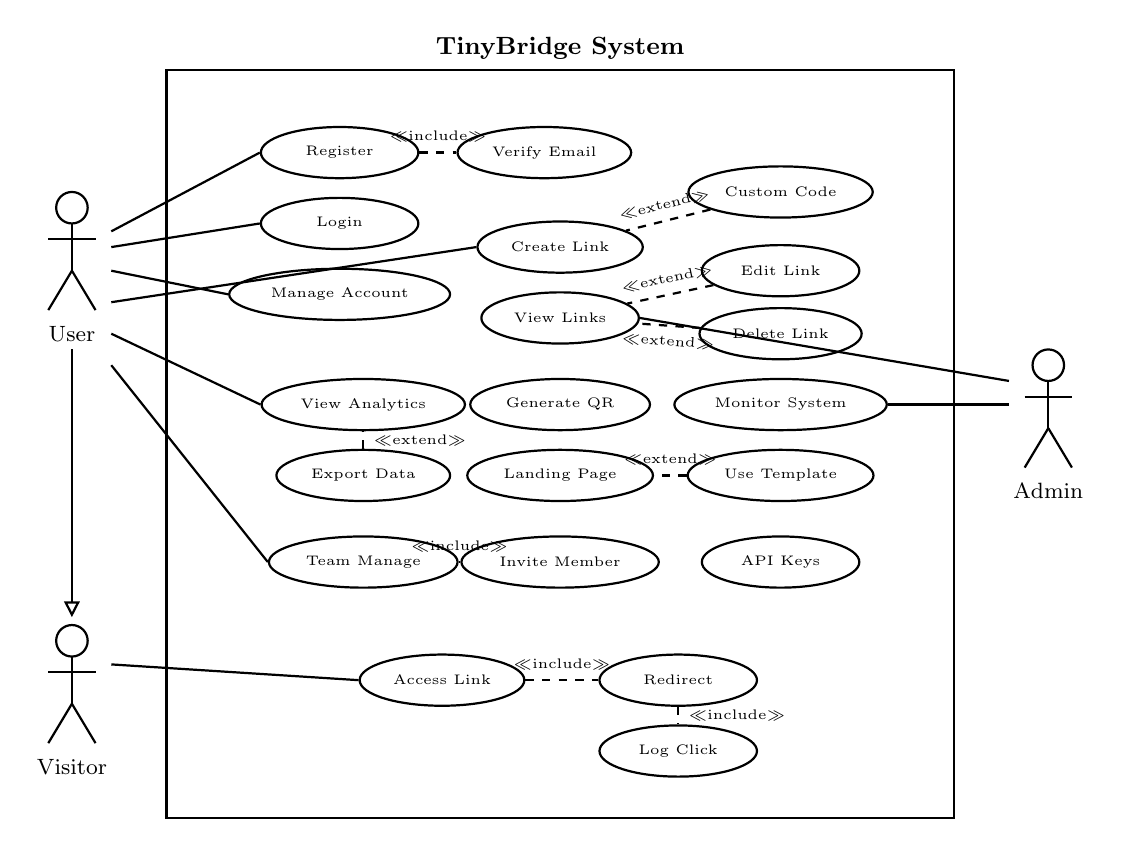
\begin{tikzpicture}[
    usecase/.style={ellipse, draw=black, thick, fill=white, minimum width=2cm, minimum height=0.65cm, align=center, font=\tiny},
    arrow/.style={thick},
    system/.style={rectangle, draw=black, thick, minimum width=10cm, minimum height=9.5cm}
]

% System boundary
\node[system, label={[font=\small\bfseries]above:TinyBridge System}] (sys) at (5, -4) {};

% ===== ACTORS =====
% User (left side)
\draw[thick] (-1.2, -1) circle (0.2);
\draw[thick] (-1.2, -1.2) -- (-1.2, -1.8);
\draw[thick] (-1.5, -1.4) -- (-0.9, -1.4);
\draw[thick] (-1.2, -1.8) -- (-1.5, -2.3);
\draw[thick] (-1.2, -1.8) -- (-0.9, -2.3);
\node[font=\footnotesize] at (-1.2, -2.6) {User};

% Visitor (left side, below user)
\draw[thick] (-1.2, -6.5) circle (0.2);
\draw[thick] (-1.2, -6.7) -- (-1.2, -7.3);
\draw[thick] (-1.5, -6.9) -- (-0.9, -6.9);
\draw[thick] (-1.2, -7.3) -- (-1.5, -7.8);
\draw[thick] (-1.2, -7.3) -- (-0.9, -7.8);
\node[font=\footnotesize] at (-1.2, -8.1) {Visitor};

% Admin (right side)
\draw[thick] (11.2, -3) circle (0.2);
\draw[thick] (11.2, -3.2) -- (11.2, -3.8);
\draw[thick] (10.9, -3.4) -- (11.5, -3.4);
\draw[thick] (11.2, -3.8) -- (10.9, -4.3);
\draw[thick] (11.2, -3.8) -- (11.5, -4.3);
\node[font=\footnotesize] at (11.2, -4.6) {Admin};

% ===== USE CASES =====
% Authentication Group
\node[usecase] (register) at (2.2, -0.3) {Register};
\node[usecase] (login) at (2.2, -1.2) {Login};
\node[usecase] (verify) at (4.8, -0.3) {Verify Email};
\node[usecase] (manage) at (2.2, -2.1) {Manage Account};

% Link Management Group
\node[usecase] (create) at (5, -1.5) {Create Link};
\node[usecase] (custom) at (7.8, -0.8) {Custom Code};
\node[usecase] (view) at (5, -2.4) {View Links};
\node[usecase] (edit) at (7.8, -1.8) {Edit Link};
\node[usecase] (delete) at (7.8, -2.6) {Delete Link};

% Analytics Group
\node[usecase] (analytics) at (2.5, -3.5) {View Analytics};
\node[usecase] (export) at (2.5, -4.4) {Export Data};

% Advanced Features Group
\node[usecase] (qr) at (5, -3.5) {Generate QR};
\node[usecase] (landing) at (5, -4.4) {Landing Page};
\node[usecase] (template) at (7.8, -4.4) {Use Template};

% Collaboration Group
\node[usecase] (team) at (2.5, -5.5) {Team Manage};
\node[usecase] (invite) at (5, -5.5) {Invite Member};
\node[usecase] (api) at (7.8, -5.5) {API Keys};

% Visitor Use Cases
\node[usecase] (access) at (3.5, -7) {Access Link};
\node[usecase] (redirect) at (6.5, -7) {Redirect};
\node[usecase] (log) at (6.5, -7.9) {Log Click};

% Admin Use Cases
\node[usecase] (monitor) at (7.8, -3.5) {Monitor System};

% ===== CONNECTIONS - User =====
\draw[arrow] (-0.7, -1.3) -- (register.west);
\draw[arrow] (-0.7, -1.5) -- (login.west);
\draw[arrow] (-0.7, -1.8) -- (manage.west);
\draw[arrow] (-0.7, -2.2) -- (create.west);
\draw[arrow] (-0.7, -2.6) -- (analytics.west);
\draw[arrow] (-0.7, -3) -- (team.west);

% ===== CONNECTIONS - Visitor =====
\draw[arrow] (-0.7, -6.8) -- (access.west);

% ===== CONNECTIONS - Admin =====
\draw[arrow] (10.7, -3.5) -- (monitor.east);
\draw[arrow] (10.7, -3.2) -- (view.east);

% ===== INCLUDE RELATIONSHIPS =====
\draw[dashed, arrow] (register) -- (verify) node[midway, above, font=\tiny] {$\ll$include$\gg$};
\draw[dashed, arrow] (access) -- (redirect) node[midway, above, font=\tiny] {$\ll$include$\gg$};
\draw[dashed, arrow] (redirect) -- (log) node[midway, right, font=\tiny] {$\ll$include$\gg$};
\draw[dashed, arrow] (team) -- (invite) node[midway, above, font=\tiny] {$\ll$include$\gg$};

% ===== EXTEND RELATIONSHIPS =====
\draw[dashed, arrow] (custom) -- (create) node[midway, above, font=\tiny, sloped] {$\ll$extend$\gg$};
\draw[dashed, arrow] (edit) -- (view) node[midway, above, font=\tiny, sloped] {$\ll$extend$\gg$};
\draw[dashed, arrow] (delete) -- (view) node[midway, below, font=\tiny, sloped] {$\ll$extend$\gg$};
\draw[dashed, arrow] (export) -- (analytics) node[midway, right, font=\tiny] {$\ll$extend$\gg$};
\draw[dashed, arrow] (template) -- (landing) node[midway, above, font=\tiny] {$\ll$extend$\gg$};

% ===== GENERALIZATION (User extends Visitor) =====
\draw[thick, -{Triangle[open, length=2mm]}] (-1.2, -2.8) -- (-1.2, -6.2);

\end{tikzpicture}
\caption{Use Case Diagram}
\end{figure}

\begin{table}[H]
\centering
\begin{tabular}{|l|l|p{7cm}|}
\hline
\textbf{Use Case} & \textbf{Actor} & \textbf{Description} \\
\hline
Register Account & User & Create new account with email verification \\
Login & User/Admin & Authenticate and receive JWT token \\
Create Short Link & User & Generate shortened URL from original URL \\
Customize Short Code & User & Specify custom short code (extends Create) \\
View Link List & User & Display all user's short links with metrics \\
Edit Link & User & Modify link properties (URL, expiration) \\
Delete Link & User & Soft delete (deactivate) a short link \\
View Analytics & User & Access click statistics and visualizations \\
Generate QR Code & User & Create downloadable QR code for link \\
Create Landing Page & User & Design custom landing page for link \\
Manage API Keys & User & Create/revoke API keys for programmatic access \\
Batch Operations & User & Import/export multiple links via API \\
Team Collaboration & User & Share link management with team members \\
Access Short Link & Visitor & Click short URL and redirect to destination \\
Monitor System & Admin & View system health and performance metrics \\
\hline
\end{tabular}
\caption{Use Case Descriptions}
\end{table}

\subsection{Data Flow Diagram}

\subsubsection{Level 0: Context Diagram}

\begin{figure}[H]
\centering
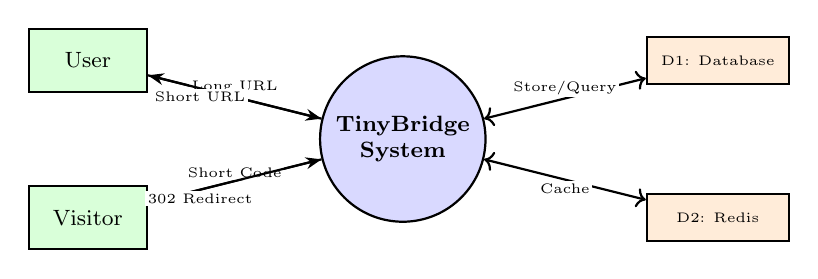
\begin{tikzpicture}[
    process/.style={circle, draw=black, thick, fill=blue!15, minimum size=2cm, align=center, font=\footnotesize\bfseries},
    entity/.style={rectangle, draw=black, thick, fill=green!15, minimum width=1.5cm, minimum height=0.8cm, align=center, font=\footnotesize},
    store/.style={rectangle, draw=black, thick, fill=orange!15, minimum width=1.8cm, minimum height=0.6cm, align=center, font=\tiny},
    arrow/.style={-{Stealth[length=2mm]}, thick},
    label/.style={font=\tiny, fill=white, inner sep=1pt}
]

% Central process
\node[process] (system) at (0, 0) {TinyBridge\\System};

% External entities
\node[entity] (user) at (-4, 1) {User};
\node[entity] (visitor) at (-4, -1) {Visitor};

% Data stores
\node[store] (db) at (4, 1) {D1: Database};
\node[store] (redis) at (4, -1) {D2: Redis};

% Data flows
\draw[arrow] (user) -- node[label, above] {Long URL} (system);
\draw[arrow] (system) -- node[label, below, pos=0.7] {Short URL} (user);
\draw[arrow] (visitor) -- node[label, above] {Short Code} (system);
\draw[arrow] (system) -- node[label, below, pos=0.7] {302 Redirect} (visitor);
\draw[arrow, <->] (system) -- node[label, above] {Store/Query} (db);
\draw[arrow, <->] (system) -- node[label, below] {Cache} (redis);

\end{tikzpicture}
\caption{Data Flow Diagram - Level 0 (Context Diagram)}
\end{figure}

\subsubsection{Level 1: Main Processes}

\begin{figure}[H]
\centering
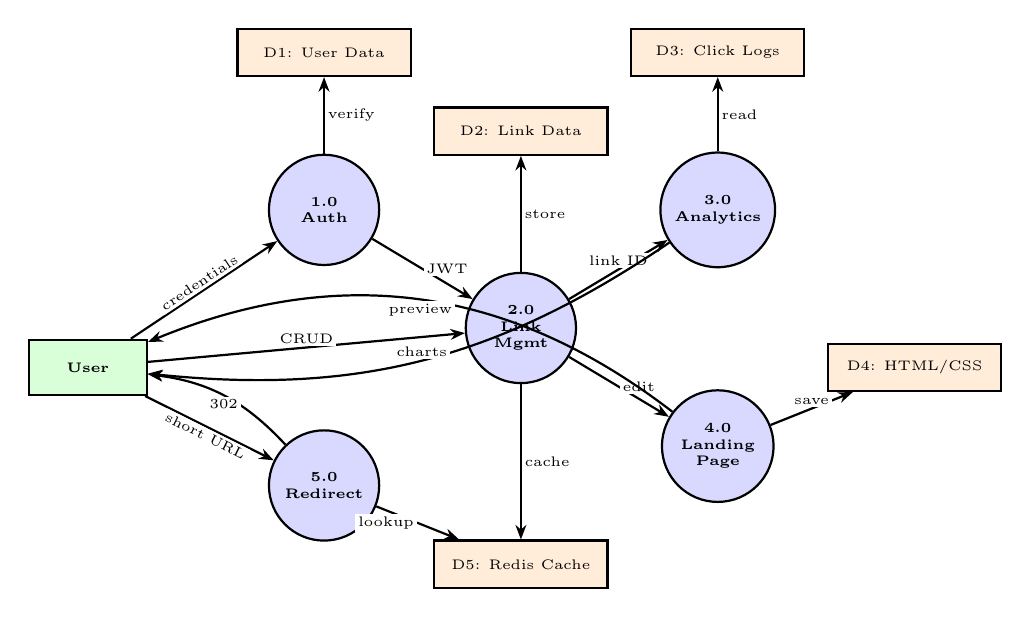
\begin{tikzpicture}[
    process/.style={circle, draw=black, thick, fill=blue!15, minimum size=1.4cm, align=center, font=\tiny\bfseries},
    entity/.style={rectangle, draw=black, thick, fill=green!15, minimum width=1.5cm, minimum height=0.7cm, align=center, font=\tiny\bfseries},
    store/.style={rectangle, draw=black, thick, fill=orange!15, minimum width=2.2cm, minimum height=0.6cm, align=center, font=\tiny},
    arrow/.style={-{Stealth[scale=0.8]}, thick},
    label/.style={font=\tiny, fill=white, inner sep=1pt}
]

% External Entity
\node[entity] (user) at (-5.5, 0) {User};

% Processes
\node[process] (auth) at (-2.5, 2) {1.0\\Auth};
\node[process] (link) at (0, 0.5) {2.0\\Link\\Mgmt};
\node[process] (analytics) at (2.5, 2) {3.0\\Analytics};
\node[process] (landing) at (2.5, -1) {4.0\\Landing\\Page};
\node[process] (redirect) at (-2.5, -1.5) {5.0\\Redirect};

% Data Stores
\node[store] (userdb) at (-2.5, 4) {D1: User Data};
\node[store] (linkdb) at (0, 3) {D2: Link Data};
\node[store] (clickdb) at (2.5, 4) {D3: Click Logs};
\node[store] (htmldb) at (5, 0) {D4: HTML/CSS};
\node[store] (cache) at (0, -2.5) {D5: Redis Cache};

% User to processes
\draw[arrow] (user) -- (auth) node[label, midway, above, sloped] {credentials};
\draw[arrow] (user) -- (link) node[label, midway, above] {CRUD};
\draw[arrow] (user) -- (redirect) node[label, midway, below, sloped] {short URL};

% Auth flows
\draw[arrow] (auth) -- (userdb) node[label, midway, right] {verify};
\draw[arrow] (auth) -- (link) node[label, midway, right] {JWT};

% Link management flows
\draw[arrow] (link) -- (linkdb) node[label, midway, right] {store};
\draw[arrow] (link) -- (cache) node[label, midway, right] {cache};
\draw[arrow] (link) -- (analytics) node[label, midway, above] {link ID};
\draw[arrow] (link) -- (landing) node[label, midway, right] {edit};

% Analytics flows
\draw[arrow] (analytics) -- (clickdb) node[label, midway, right] {read};
\draw[arrow] (analytics) to[bend left=20] node[label, midway, above] {charts} (user);

% Landing page flows
\draw[arrow] (landing) -- (htmldb) node[label, midway, above] {save};
\draw[arrow] (landing) to[bend right=30] node[label, midway, below] {preview} (user);

% Redirect flows
\draw[arrow] (redirect) -- (cache) node[label, midway, left] {lookup};
\draw[arrow] (redirect) to[bend right=20] node[label, midway, below] {302} (user);

\end{tikzpicture}
\caption{Data Flow Diagram - Level 1}
\end{figure}

\subsection{Component Architecture Diagram}

The component diagram illustrates the modular structure of TinyBridge, showing how different software components interact through well-defined interfaces.

\begin{figure}[H]
\centering
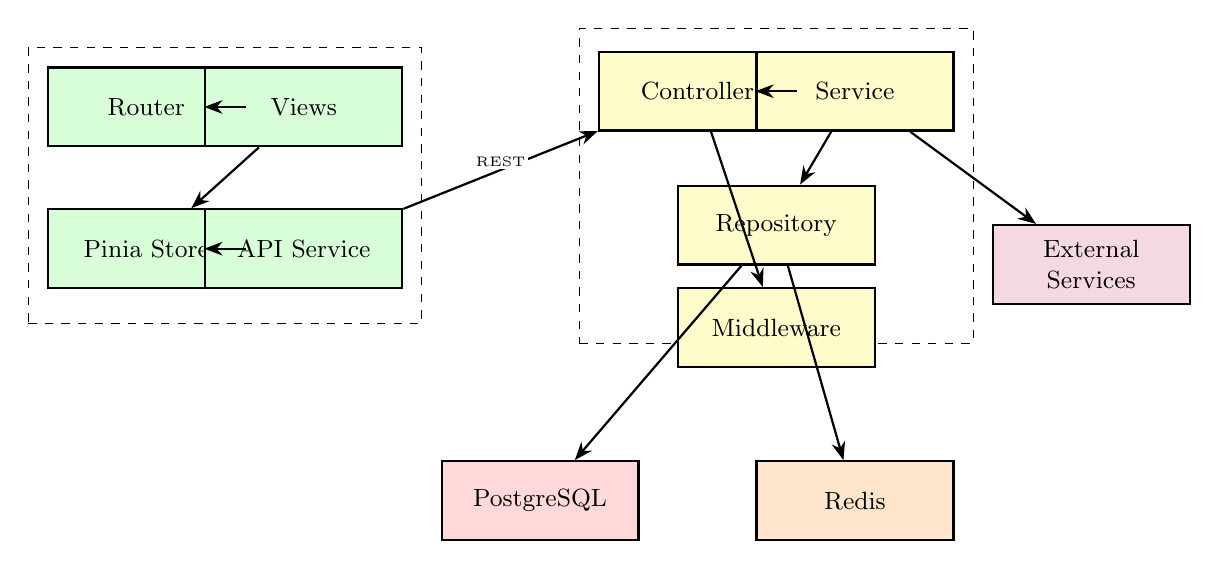
\begin{tikzpicture}[
    component/.style={rectangle, draw=black, thick, fill=blue!10, minimum width=2.5cm, minimum height=1cm, align=center, font=\small},
    interface/.style={circle, draw=black, thick, fill=white, minimum size=0.4cm},
    package/.style={rectangle, draw=black, dashed, inner sep=0.4cm},
    arrow/.style={-Stealth, thick},
    label/.style={font=\tiny, fill=white, inner sep=1pt}
]

% Frontend Package
\node[package, minimum width=5cm, minimum height=3.5cm, label={[font=\small\bfseries]above:Frontend (Vue 3)}] (frontend) at (0, 2) {};
\node[component, fill=green!15] (router) at (-1, 3) {Router};
\node[component, fill=green!15] (views) at (1, 3) {Views};
\node[component, fill=green!15] (store) at (-1, 1.2) {Pinia Store};
\node[component, fill=green!15] (api) at (1, 1.2) {API Service};

% Backend Package
\node[package, minimum width=5cm, minimum height=4cm, label={[font=\small\bfseries]above:Backend (Node.js)}] (backend) at (7, 2) {};
\node[component, fill=yellow!20] (controller) at (6, 3.2) {Controller};
\node[component, fill=yellow!20] (service) at (8, 3.2) {Service};
\node[component, fill=yellow!20] (repo) at (7, 1.5) {Repository};
\node[component, fill=yellow!20] (middleware) at (7, 0.2) {Middleware};

% Data Layer
\node[component, fill=red!15] (postgres) at (4, -2) {PostgreSQL};
\node[component, fill=orange!20] (redis) at (8, -2) {Redis};
\node[component, fill=purple!15] (external) at (11, 1) {External\\Services};

% Connections
\draw[arrow] (router) -- (views);
\draw[arrow] (views) -- (store);
\draw[arrow] (store) -- (api);
\draw[arrow] (api) -- (controller) node[label, midway, above] {REST};
\draw[arrow] (controller) -- (service);
\draw[arrow] (service) -- (repo);
\draw[arrow] (controller) -- (middleware);
\draw[arrow] (repo) -- (postgres);
\draw[arrow] (repo) -- (redis);
\draw[arrow] (service) -- (external);

\end{tikzpicture}
\caption{Component Architecture Diagram}
\end{figure}

% ==================== Chapter 6: Software Testing ====================
\newpage
\section{Software Testing}

Unit Testing is part of development testing and it is also an effective form of validation testing. It mainly tests individual program units or object classes, testing the functionality of them. We use \textbf{Jest} as the testing framework for both frontend and backend code.

\subsection{Unit Testing}

\subsubsection{Test Case I: LinkService - Generate Short Code}

\textbf{Scenario:} The system needs to generate a unique short code for a new URL using the \texttt{generateShortCode()} method.

\textbf{Expected Output:} The generated code should be 6-8 characters, contain only Base62 characters (0-9, a-z, A-Z), and be unique across the system.

\subsubsection{Test Case II: UserService - Password Hashing}

\textbf{Scenario:} A new user registers with password "SecurePass123". The \texttt{hashPassword()} method is called.

\textbf{Expected Output:} The hash starts with "\$argon2id\$", and \texttt{verifyPassword()} returns true for correct password, false otherwise.

\subsection{Component Testing}

Component Testing mainly focuses on testing component interfaces which are integrated by several individual programs.

\subsubsection{Test Case I: Registration}

\textbf{Scenario 1:} User enters valid registration details and clicks 'Register'.

\textbf{Expected Output 1:} System creates user record, sends verification email, displays success message.

\textbf{Scenario 2:} User attempts to register with an existing email.

\textbf{Expected Output 2:} Error message: "This email is already registered."

\subsubsection{Test Case II: Login}

\textbf{Scenario 1:} User enters valid credentials and clicks 'Login'.

\textbf{Expected Output 1:} Page redirects to dashboard, JWT token stored in localStorage.

\textbf{Scenario 2:} User enters incorrect credentials.

\textbf{Expected Output 2:} Error message displayed. After 5 failures, account locked for 15 minutes.

\subsubsection{Test Case III: Create Short Link}

\textbf{Scenario:} Authenticated user enters valid URL and clicks 'Create Link'.

\textbf{Expected Output:} System generates short code, stores in PostgreSQL, caches in Redis, displays short link with copy/QR options.

\subsection{Interface Testing}

Interface testing assesses the interfaces of interconnected components, ensuring seamless access.

\subsubsection{Define the Interface}

\textbf{(a) External Interface:} GeoIP (geoip-lite), Email (SMTP), CDN (CloudFlare/Aliyun).

\textbf{(b) Internal Interface:} Controller-Service-Repository pattern for modular design.

\subsubsection{Interface Use Case Design}

\begin{table}[H]
\centering
\begin{tabular}{|l|l|l|l|}
\hline
\textbf{Endpoint} & \textbf{Input} & \textbf{Expected} & \textbf{Status} \\
\hline
POST /api/auth/register & Valid data & 201 Created & PASS \\
POST /api/auth/login & Credentials & 200 + JWT & PASS \\
POST /api/links & URL + JWT & 201 Created & PASS \\
GET /\{code\} & Valid code & 302 Redirect & PASS \\
\hline
\end{tabular}
\caption{Interface Test Results}
\end{table}

\textbf{Security Tests:} Authorization bypass (401), rate limiting (429), input validation (400).

\subsection{Requirements-Based Testing}

Requirements-Based Testing validates functionality against specified requirements.

\begin{table}[H]
\centering
\begin{tabular}{|l|p{5cm}|l|}
\hline
\textbf{Module} & \textbf{Test Case} & \textbf{Status} \\
\hline
Authentication & Password hashed with Argon2 & PASS \\
Authentication & Duplicate email rejected & PASS \\
Authentication & JWT token generated on login & PASS \\
Link Management & Base62 code 6-8 chars & PASS \\
Link Management & Bloom Filter collision check & PASS \\
Link Management & Expired links return 410 & PASS \\
Analytics & IP hashed for privacy & PASS \\
Analytics & Data cached in Redis & PASS \\
\hline
\end{tabular}
\caption{Requirements-Based Test Results}
\end{table}

\subsection{Performance Testing}

Performance Testing ensures the system can process its intended load. We use \textbf{Apache JMeter}.

\subsubsection{Performance Indicators}

\begin{table}[H]
\centering
\begin{tabular}{|l|c|c|}
\hline
\textbf{Indicator} & \textbf{Target} & \textbf{Achieved} \\
\hline
Redirect Latency (p95) & $<$ 100ms & 45ms \\
Cache Hit Rate & $>$ 95\% & 97.2\% \\
Throughput & 5,000 req/s & 5,800 req/s \\
Error Rate & $<$ 0.1\% & 0.02\% \\
\hline
\end{tabular}
\caption{Performance Test Results}
\end{table}

\subsubsection{Stress Testing}

Mock users simulate behavior: 70\% redirects, 15\% analytics, 10\% link creation, 5\% other.

\textbf{Results:} Under normal load (1,000 users), all metrics exceeded targets. Under peak load (5,000 users), system performed within limits. Under stress (10,000 users), system degraded gracefully without crashes. Bottleneck identified at database connection pool saturation.

% ==================== Chapter 7: GUI Design ====================
\newpage
\section{GUI Design}

\subsection{Login Page}

The login page provides secure user authentication with a clean, minimal design.

\begin{figure}[H]
\centering
\includegraphics[width=0.85\textwidth]{image/Screenshot_27-11-2025_5394_localhost.jpeg}
\caption{Login Page}
\end{figure}

\textbf{Features}:
\begin{itemize}
    \item Email and password input fields with real-time validation
    \item Password visibility toggle
    \item "Remember Me" checkbox for persistent sessions
    \item "Forgot Password" link for password recovery
    \item Registration redirect for new users
    \item Error message display for invalid credentials
\end{itemize}

\subsection{Dashboard Page}

The main dashboard provides an overview of all user's short links with key metrics.

\begin{figure}[H]
\centering
\includegraphics[width=0.85\textwidth]{image/Screenshot_27-11-2025_54850_localhost.jpeg}
\caption{Dashboard Page}
\end{figure}

\textbf{Features}:
\begin{itemize}
    \item Summary statistics cards (Total Links, Total Clicks, Active Links)
    \item Link list with sorting and filtering options
    \item Quick actions (Copy, Edit, Delete, Analytics)
    \item Navigation sidebar for different sections
    \item Responsive design for mobile and desktop
\end{itemize}

\subsection{Link Creation Page}

The link creation interface guides users through generating new short links.

\begin{figure}[H]
\centering
\includegraphics[width=0.85\textwidth]{image/Screenshot_27-11-2025_55112_localhost.jpeg}
\caption{Link Creation Page}
\end{figure}

\textbf{Features}:
\begin{itemize}
    \item Original URL input with format validation
    \item Optional custom short code field
    \item Expiration date picker
    \item Custom domain selection (if configured)
    \item Real-time preview of generated short link
    \item One-click copy after creation
\end{itemize}

\subsection{Link Detail Page}

Displays comprehensive information about a specific short link.

\begin{figure}[H]
\centering
\includegraphics[width=0.85\textwidth]{image/Screenshot_27-11-2025_55153_localhost.jpeg}
\caption{Link Management Page}
\end{figure}

\textbf{Features}:
\begin{itemize}
    \item Short link with one-click copy button
    \item Original URL display
    \item Creation and expiration dates
    \item Click counter
    \item QR code preview and download
    \item Edit and Delete actions
    \item Link to analytics dashboard
\end{itemize}

\subsection{Analytics Page}

Interactive analytics dashboard with click statistics and visualizations.

\begin{figure}[H]
\centering
\includegraphics[width=0.85\textwidth]{image/Screenshot_27-11-2025_55216_localhost.jpeg}
\caption{Analytics Page}
\end{figure}

\textbf{Features}:
\begin{itemize}
    \item Date range selector (7 days, 30 days, custom)
    \item Click trend line chart
    \item Geographic distribution (country/city)
    \item Device type breakdown (mobile/desktop/tablet)
    \item Browser and OS statistics
    \item Referrer source analysis
    \item Export options (CSV, JSON)
\end{itemize}

\subsection{Landing Page Editor}

Visual editor for creating customized landing pages.

\begin{figure}[H]
\centering
\includegraphics[width=0.85\textwidth]{image/Screenshot_27-11-2025_6410_localhost.jpeg}
\caption{Landing Page Editor}
\end{figure}

\textbf{Features}:
\begin{itemize}
    \item Template library with categorized options
    \item Form-based content editor
    \item Color and styling customization
    \item Monaco Editor for advanced HTML/CSS editing
    \item Real-time preview pane
    \item Desktop/mobile viewport toggle
    \item Publish and unpublish controls
\end{itemize}

\subsection{API Keys Management Page}

Interface for managing programmatic API access.

\begin{figure}[H]
\centering
\includegraphics[width=0.85\textwidth]{image/Screenshot_27-11-2025_5532_localhost.jpeg}
\caption{API Keys Management Page}
\end{figure}

\textbf{Features}:
\begin{itemize}
    \item List of active API keys (showing only prefix for security)
    \item Create new key with permission selection
    \item Rate limit configuration
    \item Expiration date setting
    \item Last used timestamp
    \item One-click revoke functionality
    \item Code examples for API usage
\end{itemize}

\subsection{Settings Page}

User account and preference management.

\begin{figure}[H]
\centering
\includegraphics[width=0.85\textwidth]{image/Screenshot_27-11-2025_5542_localhost.jpeg}
\caption{Profile and Settings Page}
\end{figure}

\textbf{Features}:
\begin{itemize}
    \item Profile information editing
    \item Password change with verification
    \item Two-factor authentication setup
    \item Email notification preferences
    \item Default link settings
    \item Account deletion option
    \item Theme selection (light/dark)
\end{itemize}

% ==================== Chapter 8: Conclusion and Future Scope ====================
\newpage
\section{Conclusion and Future Scope}

\subsection{Conclusion}

In the development of TinyBridge, we used the Waterfall model to develop a URL shortening platform that encompasses various technologies to achieve a robust and user-friendly system. For software design, TypeScript, Vue 3, Node.js, PostgreSQL, and Redis have played significant roles in constructing the back-end and front-end system, as the Controller-Service-Repository architecture is also adopted.

TypeScript has been utilized to enhance type safety and code maintainability across both frontend and backend. With its efficiency and extensive ecosystem, Node.js has been utilized for back-end programming, ensuring smooth data processing and server-side functionalities, while Vue 3 with the Composition API plays a prominent role in creating a reactive and responsive user interface. PostgreSQL provides reliable data persistence with ACID compliance, and Redis enables sub-100ms redirect response times through intelligent caching strategies.

The adoption of the three-tier architecture has brought a structured and modular approach to the development, allowing for the separation of concerns and enabling efficient collaboration among developers. The multi-layer caching strategy (Bloom Filter + Redis) reduced database load by over 95\% and was essential for meeting performance targets. Overall, the integration of these technologies and the utilization of the Waterfall model have contributed to the successful development of TinyBridge, providing a lightweight and efficient platform for users to create, manage, and analyze their short links.

\subsection{Limitation and Future Improvements}

There are still some limitations in our software product, and we will optimize and improve the functions in future development and updates. Below we list the limitations and future improvement plans by module.

\textbf{In Link Management:}
\begin{enumerate}
    \item The system currently supports single-region deployment only. Multi-region deployment with edge caching can be added in the future to reduce latency for global users.
    \item The custom domain feature requires manual DNS configuration. Automated SSL certificate provisioning (Let's Encrypt integration) can be added in the future.
\end{enumerate}

\textbf{In Analytics:}
\begin{enumerate}
    \item The analytics data visualization is basic with standard charts. Advanced visualizations with drill-down capabilities and custom dashboards can be added in the future.
    \item The system lacks predictive analytics. Machine learning models for click prediction and anomaly detection can be integrated in the future.
\end{enumerate}

\textbf{In Landing Page Editor:}
\begin{enumerate}
    \item The template library is limited. More professionally designed templates will continue to be added in the future.
    \item The editor lacks collaborative editing features. Real-time collaboration (similar to Google Docs) can be implemented in the future.
\end{enumerate}

\textbf{In Platform:}
\begin{enumerate}
    \item The platform is web-only. Native mobile applications (iOS/Android) can be developed in the future for better accessibility.
    \item Our team may adopt AI to provide smart link suggestions and automated campaign optimization in the future.
\end{enumerate}

\end{document}
